\documentclass[fleqn,10pt]{article}

% Scientific Data template
\usepackage[utf8]{inputenc}
\usepackage{graphicx}
\usepackage{amsmath}
\usepackage{booktabs}
\usepackage{hyperref}
\usepackage[margin=2.5cm]{geometry}
\usepackage{siunitx}
\usepackage{authblk}
\usepackage{ragged2e}
\usepackage{enumitem}
\usepackage{upquote}
\usepackage{tikz}
\usetikzlibrary{shapes.geometric, arrows.meta, positioning, calc}

%QMEnum-2-3 is the working name of the dataset
\title{Quantum chemistry calculations from systematic enumeration of small molecule structures}

\author[1]{Gábor János Tornai}
\author[1]{Álex Kálmán Balogh}
\author[1]{Ádám Rák}
\author[2]{György Cserey}
\affil[1]{StreamNovation Ltd.}
\affil[2]{Pázmány Péter Catholic University, Faculty of Information Technology and Bionics}

\date{\today}


\begin{document}
\maketitle

\begin{abstract}
We present a quantum chemistry dataset providing non-equilibrium geometries, atomic forces, density matrices, and molecular orbital coefficients for 112,958 systematically enumerated small molecules across 338,616 calculations. Unlike geometry-optimized datasets, where forces vanish identically at equilibrium, structures here were pre-relaxed using the Universal Force Field (UFF), preserving meaningful atomic forces suitable for training force-predicting machine learning models. Generated through combinatorial enumeration across all 18 elements of the first three periods (H through Ar), the dataset encompasses neutral, charged ($\pm 1, \pm 2$), radical, high-spin, noble gas-containing, and unusual-valence species, with a single, maximum-multiplicity spin state per specification, spanning geometries from near-equilibrium to heavily strained configurations. Each electronic structure specification was computed with three of the nine combinations of three methods (Hartree-Fock, B3LYP, $\omega$B97X-D) and three basis sets (STO-3G, 6-31G*, DEF2-SVP), selected such that each method and each basis set appears exactly once. The dataset comprises two subsets: 2,960 molecules with 2 heavy atoms (8,973 calculations) and 109,998 molecules with 3 heavy atoms (329,643 calculations).

\textbf{Keywords:} quantum chemistry, machine learning, molecular dataset, density functional theory, electronic structure, atomic force
\end{abstract}
%----------------------------------------------------------------
\section*{Background \& Summary}

Machine learning methods for predicting quantum chemical properties have shown promise for accelerating electronic structure calculations\cite{schuett2019, neurips2021, bigdata_bde}. Training reliable models requires benchmark datasets that systematically sample chemical space across diverse compositions, charge states, and nuclear configurations. In particular, developing machine learning potentials and force-prediction architectures demands non-equilibrium geometries where atomic forces do not vanish, while electronic-structure-level ML tasks (such as predicting density matrices or molecular orbital coefficients) rely on standard Gaussian-type orbital (GTO) representations.

Early molecular benchmarks, such as QM7\cite{QM7} and QM9\cite{QM9}, primarily provided equilibrium geometries of neutral, closed-shell organic molecules computed at a single level of theory. Subsequent efforts broadened this scope: datasets such as ANI-1\cite{smith2017ani} introduced non-equilibrium normal-mode sampling; ANI-1x\cite{smith2020ani} and SPICE\cite{eastman2023spice, spice2} supplied atomic forces for conformational and thermal fluctuations in organic and drug-like systems; QMugs\cite{qmugs} and PubChemQC\cite{pubchemqc, pubchemqc2023b3lyp} delivered large-scale electronic structure data; and QCML\cite{qcml} scaled sampling to tens of millions of configurations from semi-empirical thermal exploration across dozens of elements (Table~\ref{tab:comparison}).

However, existing resources predominantly focus on conformational sampling of moderate-sized organic frameworks, where elemental diversity outside the organic subset (H, C, N, O, S, P) and non-standard electronic states (radicals, high spin, unusual formal oxidation states) appear only sparsely, if at all. For example, while QCML samples 79 elements, periods 1--3 noble gases are absent, alkali and alkaline-earth metals occur in a fraction of structures below approximately $10^{-6}$, and spin multiplicities are restricted to singlets and doublets. Rather than competing with extensive conformational libraries of larger molecules, the present dataset operates in a distinct, complementary regime: systematic combinatorial enumeration of small (2--3 heavy atom) frameworks across elemental, charge, and bonding space, with a single non-equilibrium geometry per molecule.

\begin{table}[ht!]
\centering
\resizebox{\textwidth}{!}{
\begin{tabular}{lccccccll}
\toprule
Dataset & \#Elements & Charge range & Max.~mult. & Forces & Density/MO & Basis type & Geometry source & \#Geometries \\
\midrule
This work & 18 & $-2\ldots+2$ & 7 & Yes & Yes & GTO & UFF, 50 it. (non-eq) & 112,958$^{a}$ \\
QCML~\cite{qcml} & 79$^{b}$ & $-2\ldots+2$ & 2 & Yes & Yes & NAO & semi-emp. thermal sampling (0--1000 K) & 33.5M \\
ANI-1~\cite{smith2017ani} & 4 & 0 & 1 & No & No & GTO & DFT opt.\ + normal mode sampling (non-eq) & 22.1M \\
ANI-1x~\cite{smith2020ani} & 4 & 0 & 1 & Yes & No & GTO & Active learning / MD (non-eq) & 4.96M \\
SPICE 1~\cite{eastman2023spice} & 15 & $-1\ldots+1$ & 1 & Yes & No & GTO & MD, conformers \& ion pairs (non-eq) & 1.13M \\
SPICE 2~\cite{spice2} & 17 & $-1\ldots+1$ & 1 & Yes & No & GTO & MD thermal sampling (non-eq) & 2.0M \\
QMugs~\cite{qmugs} & 10 & 0 & 1 & No & Yes & GTO & GFN2-xTB MTD + opt.\ (minima) & 1.99M \\
OC20~\cite{oc20} & 55 & 0 & 1 & Yes & No & PW & DFT relax.\ + AIMD + rattled (non-eq) & $\sim$250M \\
PubChemQC~\cite{pubchemqc} & 12 & 0 & 1 & No & Yes & GTO & PM6 equilibrium & 3M \\
PubChemQC B3LYP//PM6~\cite{pubchemqc2023b3lyp} & 71 & 0 & 1 & No & Yes & GTO & PM6 equilibrium & 86M \\
GEOM~\cite{geom} & 9 & $-1\ldots+2$ & 1 & No & No & GTO & conformers, MD thermal sampling & 37M \\
Alexandria~\cite{alexandria} & 26 & $-4\ldots+1$ & 3 & No & No & GTO & DFT equilibrium & 2,704 \\
VQM24~\cite{vqm24} & 9 & 0 & 1 & No & Yes & GTO & generated + conformers & 836k \\
OMol25~\cite{levine2025open} & 83 & $-10\ldots+10$ & 11 & Yes & Yes & GTO & various & 83M \\
QM7-X~\cite{qm7-x} & 6 & 0 & 1 & Yes & No & NAO & DFT opt.\ + normal mode sampling (1500 K) & 4.2M \\
\bottomrule
\end{tabular}
}
\vspace{1ex}

\par
\begin{minipage}{\linewidth}
\footnotesize\justifying
$^{a}$ Unique nuclear geometries; typically three calculations per geometry (one per method and per basis set; multiple graph-level specifications), 338,616 calculations in total.

$^{b}$ Number of elements occurring in at least one structure (79 of the 85 elements with $Z<86$); the majority of structures contain only H, C, N, O, S and P, noble gases of periods 1--3 are absent, and alkali and alkaline-earth metals occur in a fraction of structures below approximately $10^{-6}$.
\end{minipage}
\caption{Comparison of the present dataset with representative quantum chemistry datasets used in machine learning.}
\label{tab:comparison}
\end{table}

To address this gap, here we report quantum chemical calculations for 112,958 small molecules systematically generated through combinatorial enumeration. The dataset encompasses all 18 elements from the first three periods of the periodic table (H through Ar), including neutral, charged ($\pm 1, \pm 2$), radical, and noble-gas-containing species, with a single, maximum-multiplicity spin state per specification. In the 3-node subset, every element from H to Ar is present in at least 2.3\% of the structures, and spin multiplicities reach up to 7 (see Data Overview). The dataset is partitioned into two subsets: 2,960 molecules with 2 heavy atoms (8,973 calculations) and 109,998 molecules with 3 heavy atoms (329,643 calculations). Here, a ``node'' refers strictly to a non-hydrogen (heavy) atom in the molecular graph, with hydrogen atoms treated implicitly during graph generation. For each electronic structure specification, three calculations were performed across nine possible combinations of three methods (Hartree-Fock, B3LYP, $\omega$B97X-D) and three basis sets (STO-3G, 6-31G*, DEF2-SVP), selected such that each method and each basis set appears exactly once (see Methods).

Molecular geometries were obtained through force-field pre-relaxation with UFF rather than full quantum mechanical energy minimization, producing non-equilibrium configurations of strained and unusual-valence small molecules. Atomic force magnitudes span a wide range from near-zero values to more than 100~Ha/Bohr, capturing restoring forces and including strongly compressed geometries that reach the short-range repulsive region where close nuclear contacts provide training signals for machine learning potentials. Furthermore, for 6,279 geometries (5.6\% of the dataset), several graph-level specifications (differing in bond orders and formal charges, but sharing the same total charge and spin multiplicity) yielded identical 3D nuclear coordinates and therefore identical quantum chemical inputs; these are indexed under a single geometry entry.

Potential reuse applications for this dataset include developing and evaluating machine learning potentials and force fields on non-equilibrium geometries, analyzing electronic properties (density matrices, orbital coefficients) across diverse spin and charge regimes, and comparing aggregate behavior across Hartree-Fock and density functional approximations.

%------------------------------------------------------------------

\section*{Methods}

\begin{figure*}[htbp]
\centering
\resizebox{\textwidth}{!}{%
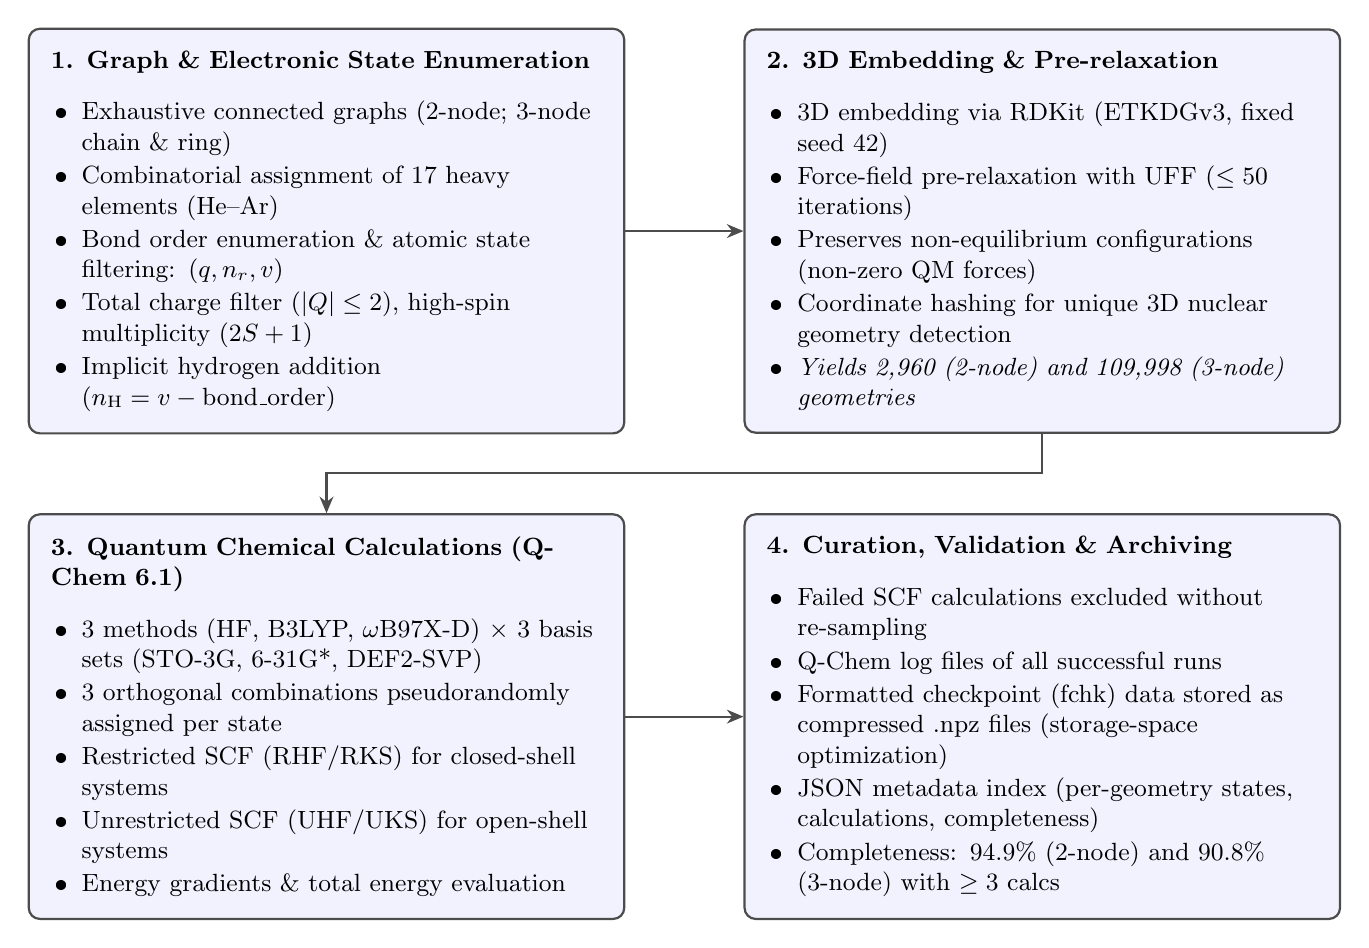
\begin{tikzpicture}[
    node distance = 1.0cm and 1.5cm,
    box/.style = {
        rectangle,
        rounded corners=4pt,
        draw=black!70,
        thick,
        fill=blue!5,
        text width=7.0cm,
        minimum height=2.8cm,
        inner sep=8pt,
        font=\small
    },
    header/.style = {
        font=\bfseries\small,
        text=blue!90!black,
        anchor=north west,
        yshift=-4pt,
        xshift=4pt
    },
    arrow/.style = {
        -{Stealth[length=6pt, width=5pt]},
        thick,
        color=black!70
    }
]

% Step 1: Graph Enumeration
\node[box] (step1) {
    \textbf{1. Graph \& Electronic State Enumeration}\\ \vspace{0.4em}
    \begin{itemize}[leftmargin=1.2em, itemsep=1pt, topsep=2pt, parsep=0pt]
        \item Exhaustive connected graphs (2-node; 3-node chain \& ring)
        \item Combinatorial assignment of 17 heavy elements (He--Ar)
        \item Bond order enumeration \& atomic state filtering: $(q, n_r, v)$
        \item Total charge filter ($|Q| \le 2$), high-spin multiplicity ($2S+1$)
        \item Implicit hydrogen addition ($n_{\mathrm{H}} = v - \text{bond\_order}$)
    \end{itemize}
};

% Step 2: 3D Geometry
\node[box, right=of step1] (step2) {
    \textbf{2. 3D Embedding \& Pre-relaxation}\\ \vspace{0.4em}
    \begin{itemize}[leftmargin=1.2em, itemsep=1pt, topsep=2pt, parsep=0pt]
        \item 3D embedding via RDKit (ETKDGv3, fixed seed 42)
        \item Force-field pre-relaxation with UFF ($\le 50$ iterations)
        \item Preserves non-equilibrium configurations (non-zero QM forces)
        \item Coordinate hashing for unique 3D nuclear geometry detection
        \item \textit{Yields 2,960 (2-node) and 109,998 (3-node) geometries}
    \end{itemize}
};

% Step 3: QM Calculations
\node[box, below=of step1] (step3) {
    \textbf{3. Quantum Chemical Calculations (Q-Chem 6.1)}\\ \vspace{0.4em}
    \begin{itemize}[leftmargin=1.2em, itemsep=1pt, topsep=2pt, parsep=0pt]
        \item 3 methods (HF, B3LYP, $\omega$B97X-D) $\times$ 3 basis sets (STO-3G, 6-31G*, DEF2-SVP)
        \item 3 orthogonal combinations pseudorandomly assigned per state
        \item Restricted SCF (RHF/RKS) for closed-shell systems
        \item Unrestricted SCF (UHF/UKS) for open-shell systems
        \item Energy gradients \& total energy evaluation
    \end{itemize}
};

% Step 4: Dataset Curation
\node[box, right=of step3] (step4) {
    \textbf{4. Curation, Validation \& Archiving}\\ \vspace{0.4em}
    \begin{itemize}[leftmargin=1.2em, itemsep=1pt, topsep=2pt, parsep=0pt]
        \item Failed SCF calculations excluded without re-sampling
        \item Q-Chem log files of all successful runs
        \item Formatted checkpoint (fchk) data stored as compressed .npz files (storage-space optimization)
        \item JSON metadata index (per-geometry states, calculations, completeness)
        \item Completeness: $94.9\%$ (2-node) and $90.8\%$ (3-node) with $\ge 3$ calcs
    \end{itemize}
};

% Connective arrows
\draw[arrow] (step1) -- (step2);
\draw[arrow] (step2.south) -- ++(0,-0.5) -| (step3.north);
\draw[arrow] (step3) -- (step4);

\end{tikzpicture}%
}
\caption{Overview of the dataset generation and validation workflow. Molecular frameworks are exhaustively enumerated, embedded in 3D, and pre-relaxed using UFF, followed by orthogonal quantum chemical property evaluations across three methods and three basis sets.}
\label{fig:workflow_flowchart}
\end{figure*}


\subsection*{Molecular Structure Generation}

\subsubsection*{Combinatorial Enumeration}

Molecular structures were generated through systematic combinatorial enumeration of molecular graphs (Figure~\ref{fig:workflow_flowchart}). The generation process began by exhaustively enumerating all connected graphs with 2 and 3 nodes, i.e.\ the single 2-node graph and both 3-node graphs (the linear chain and the three-membered ring). For each graph topology, we combinatorially assigned the 17 non-hydrogen elements of periods 1-3 (He-Ar) to the graph nodes. Bond orders between these heavy atoms were then systematically enumerated, and hydrogen atoms were added implicitly in a later step (see below).

% Requires packages: booktabs, graphicx, amsmath
\begin{table}[htbp]
\centering
\caption{Permitted valence states ($v=1\dots6$), maximum normal valences, and associated formal charge and unpaired electron counts $(q, n_r)$ for the non-hydrogen elements of periods 1--3 (He--Ar) as defined in the molecular graph generator.}
\label{tab:element_states}
\vspace{1ex}
\resizebox{\textwidth}{!}{
\begin{tabular}{l c c llllll}
\toprule
\textbf{Element} & \textbf{$Z$} & \textbf{Max. Norm. Val.}$^{a}$ & \multicolumn{6}{c}{\textbf{Valence ($v$)}$^{b}$} \\
\cmidrule(lr){4-9}
 & & & \textbf{$v=1$} & \textbf{$v=2$} & \textbf{$v=3$} & \textbf{$v=4$} & \textbf{$v=5$} & \textbf{$v=6$} \\
\midrule
\textbf{He} & 2 & 2 & $(+1,0)$ & $(+2,0)^{c}$ &  &  &  &  \\
\textbf{Li} & 3 & 1 & $(0,0)$ &  &  &  &  &  \\
\textbf{Be} & 4 & 2 & $(+1,0)$, $(0,1)$ & $(0,0)$ &  &  &  &  \\
\textbf{B} & 5 & 4 & $(-2,0)$, $(-1,1)$, $(0,2)$ & $(-1,0)$, $(0,1)$ & $(0,0)$ & $(-1,0)$ &  &  \\
\textbf{C} & 6 & 4 &  & $(-2,0)$, $(-1,1)$, $(0,2)$ & $(-1,0)$, $(0,1)$ & $(0,0)$ &  &  \\
\textbf{N} & 7 & 4 & $(-2,0)$, $(+1,1)^{d}$, $(0,2)$ & $(-1,0)$, $(0,1)$ & $(0,0)$ & $(+1,0)$ &  &  \\
\textbf{O} & 8 & 3 & $(-1,0)$, $(0,1)$ & $(0,0)$ & $(+1,0)$ &  &  &  \\
\textbf{F} & 9 & 1 & $(0,0)$ &  &  &  &  &  \\
\textbf{Ne} & 10 & 2 & $(+1,0)$ & $(+2,0)^{c}$ &  &  &  &  \\
\textbf{Na} & 11 & 1 & $(0,0)$ &  &  &  &  &  \\
\textbf{Mg} & 12 & 2 & $(+1,0)$, $(0,1)$ & $(0,0)$ &  &  &  &  \\
\textbf{Al} & 13 & 4 & $(-2,0)$, $(-1,1)$, $(0,2)$ & $(-1,0)$, $(0,1)$ & $(0,0)$ & $(-1,0)$ &  &  \\
\textbf{Si} & 14 & 4 &  & $(-2,0)$, $(-1,1)$, $(0,2)$ & $(-1,0)$, $(0,1)$ & $(0,0)$ &  &  \\
\textbf{P} & 15 & 4 & $(-2,0)$, $(+1,1)^{d}$, $(0,2)$ & $(-1,0)$, $(0,1)$ & $(0,0)$ & $(+1,0)$ & $(0,0)$ &  \\
\textbf{S} & 16 & 3 & $(-1,0)$, $(0,1)$ & $(0,0)$ & $(+1,0)$ & $(0,0)$ &  & $(0,0)$ \\
\textbf{Cl} & 17 & 1 & $(0,0)$ &  & $(0,0)$ &  & $(0,0)$ &  \\
\textbf{Ar} & 18 & 2 & $(+1,0)$ & $(+2,0)^{c}$ &  &  &  &  \\
\bottomrule
\end{tabular}
}
\vspace{1ex}
\par
\begin{minipage}{\linewidth}
\footnotesize
$^{a}$ Maximum normal valence: for valences above this value, the bond order must equal the valence (no implicit hydrogens allowed).

$^{b}$ Valence $v$ denotes the sum of explicit bond orders and implicit hydrogens ($n_{\mathrm{H}} = v - \mathrm{bond\_order}$). Since every node of a connected graph has at least one bond, $v \geq 1$.

$^{c}$ For noble gases at $v=2$, states represent formal coordination complexes (e.g., adjacent counterions).

$^{d}$ For N and P at $v=1$, the $(+1,1)$ entry corresponds to a radical cation state present in the generator dictionary (occurring in 118 2-node and 2,845 3-node representative structures).
\end{minipage}
\end{table}

For each bonded framework, we enumerated all combinations of the atomic states $(q_i, n_{r,i})$ permitted for the given valences (Table~\ref{tab:element_states}). The total molecular charge was taken as the sum of the atomic formal charges, $Q = \sum_i q_i$; configurations with $|Q| > 2$ were discarded during generation. The spin multiplicity was set to $2S+1 = N_r + 1$, where $N_r = \sum_i n_{r,i}$ is the total number of unpaired electrons, i.e.\ all unpaired electrons were assumed parallel (high-spin configuration); low-spin states of polyradicals (e.g.\ open-shell singlets) were not considered. Hydrogen atoms were subsequently added to satisfy the chosen valence of each heavy atom ($n_{\mathrm{H}} = v - \mathrm{bond\_order}$), thereby naturally covering varying levels of hydrogen saturation for each framework.

Beyond the permitted valence-state dictionary (Table~\ref{tab:element_states}), the total-charge bound ($|Q| \le 2$), and graph-level deduplication, no thermodynamic or chemical stability filter was applied, so reactive, strained, and unusual-valence species were retained. After 3D embedding and force-field pre-relaxation (discarding structures that failed at either step), this procedure yielded 2,960 unique geometries for the 2-node subset and 109,998 unique geometries for the 3-node subset.

\subsubsection*{3D Geometry Generation and Pre-relaxation}

Initial 3D coordinates were generated with RDKit\cite{rdkit} (version 2025.03.5) by embedding each molecular graph, defined by its element types, bond orders, and formal charges, using the ETKDGv3 algorithm with a fixed random seed (42). The embedded structures were then relaxed with the Universal Force Field (UFF)\cite{uff} for at most 50 iterations, without requiring convergence. This short pre-relaxation is intended only to remove severe embedding distortions while preserving non-equilibrium geometries, rather than to locate an energy minimum. Here, UFF serves solely to generate nuclear coordinate inputs; electronic state specifications (total charge and spin multiplicity) are handled entirely by the subsequent quantum chemical calculations. Because the UFF potential energy surface differs from those of the quantum chemical methods used here, the resulting geometries are in general not stationary points at the QM level and therefore exhibit non-zero atomic forces (Figure~\ref{fig:forces}). Structures for which RDKit embedding or UFF setup failed were discarded without further attempts (per-run embedding and UFF convergence logs were not retained). Unique 3D geometries were identified by computing the MD5 hash of the whitespace-normalized Cartesian coordinate block (element symbols and positions) of each pre-relaxed structure. Because force-field pre-relaxation is insensitive to alternative Lewis-structure assignments, 6,279 geometries (5.6\% of the dataset; 145 in the 2-node and 6,134 in the 3-node subset) were produced identically by multiple graph-level specifications sharing the same total charge and spin multiplicity. In such cases, all specifications share a single geometry entry, one specification is designated as the \textquoteleft representative structure\textquoteright{} in \texttt{metadata.json}, and all specifications sharing the coordinates are listed under \texttt{alternative\_structures\_details}.

\subsection*{Quantum Chemical Calculations}

All quantum chemistry calculations were performed using Q-Chem\cite{qchem} (version 6.1.0). Calculations were performed with three quantum chemistry methods: Hartree-Fock (HF), B3LYP\cite{b3lyp} hybrid density functional, and $\omega$B97X-D\cite{wb97xd} range-separated hybrid functional with empirical dispersion. These were paired with three basis sets: STO-3G (minimal basis), 6-31G* (split-valence with polarization), and DEF2-SVP (split-valence polarized). For each specification, exactly three calculations were performed, selected pseudorandomly from the nine possible method/basis combinations such that each method and each basis set appears exactly once: the first combination was drawn uniformly from all nine, the second uniformly from the four combinations sharing neither its method nor its basis set, and the third is the remaining unique combination. This procedure samples the six valid method/basis assignments with equal probability ($1/6$), so that each individual method/basis pair is assigned to a given specification with probability $1/3$. When multiple specifications map to the same 3D geometry, their converged calculations are pooled into the single geometry directory under \texttt{available\_calculations} (keyed by \texttt{METHOD\_BASIS}), which can therefore contain more than three distinct method/basis entries (whereas identical method/basis draws on the same geometry and spin--charge state yield identical inputs and merge into one entry). A fixed pseudorandom seed (42) was used throughout the entire pipeline, including conformer embedding in RDKit and the pseudorandom method--basis assignment.


All calculations were force (gradient) calculations, providing both the total electronic energy and atomic force vectors. SCF convergence threshold was set to $10^{-8}$ a.u., maximum SCF iterations to 50, initial guess to SAD (Superposition of Atomic Densities), and SCF algorithm to Pulay DIIS (Direct Inversion in Iterative Subspace). For DFT calculations, integration grids were set to SG-1 for B3LYP and SG-2 for $\omega$B97X-D (both default Q-Chem settings). Restricted SCF (RHF/RKS) was used for closed-shell systems ($2S+1 = 1$) and unrestricted SCF (UHF/UKS) for open-shell systems ($2S+1 > 1$). Internal SCF wavefunction stability analysis was not performed; consequently, for some open-shell, radical, or unusual-valence species a converged SCF solution may correspond to a local electronic stationary point rather than the global ground state.

Calculations were considered successful if SCF converged within the iteration limit, no abnormal termination occurred, and gradient calculation completed successfully. Failed calculations (SCF non-convergence or abnormal termination) were removed individually and not re-sampled. Geometries were retained even if none of their assigned calculations succeeded (2 in the 2-node and 129 in the 3-node subset); these entries contain coordinates and metadata but no QM results. After cleanup, all calculations in the dataset successfully converged.

Completeness statistics (per unique geometry): exactly three calculations are present for 91.0\% of the 2-node geometries (2,695 of 2,960) and 86.4\% of the 3-node geometries (94,991 of 109,998); at least three are present for 94.9\% and 90.8\%, respectively. Incomplete coverage (geometries with fewer than 3 calculations) resulted from SCF convergence failures for difficult electronic structures such as certain radicals or highly charged species, which were removed during quality control.

%---------------------------------------------------------------

\section*{Data Records}

The complete dataset is available on Zenodo\cite{zenodo_doi} under a Creative Commons CC-BY 4.0 license.

\subsection*{Dataset Structure}

The dataset is organized into two main directories:

\begin{verbatim}
dataset_2node/          # 2 heavy atom molecules
  mol_000001/
    metadata.json
    HF_STO-3G.qcout
    HF_STO-3G.npz
    B3LYP_6-31G*.qcout
    B3LYP_6-31G*.npz
    WB97X-D_DEF2-SVP.qcout
    WB97X-D_DEF2-SVP.npz
  mol_000002/
  ...
  dataset_metadata.json
  molecules_with_alternatives.csv

dataset_3node/          # 3 heavy atom molecules
  [same structure]
\end{verbatim}

\subsection*{File Formats}

\subsubsection*{metadata.json}

Each molecule directory contains a \texttt{metadata.json} file with:

\begin{itemize}
\item \textbf{geometry\_hash:} (\texttt{str}) Unique identifier for the 3D geometry
\item \textbf{representative\_structure:} (\texttt{dict[str, Any]}) One of the electronic structure specifications, including:
  \begin{itemize}
  \item coordinate\_elements: (\texttt{list[str]}) Atomic symbols
  \item coordinates: (\texttt{list[list[float]]}) Atomic positions (\AA ngström) in input orientation
  \item total\_charge: (\texttt{int}) Molecular charge
  \item multiplicity: (\texttt{int}) Spin multiplicity (2S+1)
  \item molecular\_hash: (\texttt{str}) Unique identifier for this electronic structure
  \item edges: (\texttt{list[list[int]]}) Bond connectivity as atom index pairs
  \item elements: (\texttt{list[str]}) Heavy atom element symbols
  \item edge\_bonds: (\texttt{dict[str, int]}) Bond orders keyed by atom index pairs
  \item atom\_states: (\texttt{dict[str, dict[str, int]]}) Per-atom electronic state information
  \item smiles: (\texttt{str}) SMILES representation
  \end{itemize}
\item \textbf{num\_alternative\_structures:} (\texttt{int}) Number of electronic structure specifications with this geometry
\item \textbf{alternative\_molecular\_hashes:} (\texttt{list[str]}) List of all electronic structure specification identifiers
\item \textbf{alternative\_structures\_details:} (\texttt{list[dict[str, Any]]}) Detailed information about alternative specifications (if applicable, only present when \texttt{num\_\allowbreak{}alternative\_\allowbreak{}structures} $>1$)
\item \textbf{available\_calculations:} (\texttt{dict[str, dict[str, str]]}) Dictionary of completed calculations with method/basis information and file names
\item \textbf{completeness:} (\texttt{str}) Ratio string \texttt{"N/3"} relative to the baseline of three calculations per specification (e.g., \texttt{"3/3"}; values below \texttt{"3/3"} reflect excluded SCF failures, whereas values above \texttt{"3/3"}, such as \texttt{"6/3"}, occur when multiple specifications share a geometry---note that if no SCF failure occurred on such a geometry, $N$ reflects the pre-deduplication specification-level calculation count rather than the number of distinct \texttt{METHOD\_\allowbreak{}BASIS} entries in \texttt{available\_\allowbreak{}calculations}, so users should query \texttt{len(available\_\allowbreak{}calculations)} for the exact stored calculation count)
\item \textbf{note:} (\texttt{str}) Explanation if multiple electronic structures share this geometry (optional, only present when applicable)
\end{itemize}

\subsubsection*{.qcout files}

Standard Q-Chem output text files containing:
\begin{itemize}
\item Input specification
\item SCF convergence details
\item Final energy and gradient
\item Molecular orbitals
\item Population analysis
\item Timing information
\end{itemize}

\subsubsection*{.npz files}

NumPy NPZ archives containing parsed Q-Chem formatted checkpoint (\texttt{.fchk}) data. Because these are single-point force evaluations on RDKit UFF pre-relaxed geometries stored in a trajectory-compatible schema, \texttt{num\_\allowbreak{}steps} $=1$ and all per-calculation entries carry the \texttt{step\_\allowbreak{}0\_\allowbreak{}} prefix. Scalar counts and quantum numbers are stored as 0D \texttt{int32} arrays, whereas vector and matrix quantities are stored as 1D \texttt{int32} or \texttt{float32} arrays.

Key data fields include:
{\emergencystretch=2.5em
\begin{itemize}
\item \textbf{Geometry, forces, and global state:} 0D \texttt{int32} scalars \texttt{step\_\allowbreak{}0\_\allowbreak{}number\_\allowbreak{}of\_\allowbreak{}atoms}, \texttt{step\_\allowbreak{}0\_\allowbreak{}charge}, \texttt{step\_\allowbreak{}0\_\allowbreak{}multiplicity}, \texttt{step\_\allowbreak{}0\_\allowbreak{}number\_\allowbreak{}of\_\allowbreak{}electrons}, \texttt{step\_\allowbreak{}0\_\allowbreak{}number\_\allowbreak{}of\_\allowbreak{}alpha\_\allowbreak{}electrons}, and \texttt{step\_\allowbreak{}0\_\allowbreak{}number\_\allowbreak{}of\_\allowbreak{}beta\_\allowbreak{}electrons}; per-atom vectors \texttt{step\_\allowbreak{}0\_\allowbreak{}atomic\_\allowbreak{}numbers} and \texttt{step\_\allowbreak{}0\_\allowbreak{}nuclear\_\allowbreak{}charges}; and 1D vectors (length $3N_{\mathrm{atoms}}$) \texttt{step\_\allowbreak{}0\_\allowbreak{}current\_\allowbreak{}cartesian\_\allowbreak{}coordinates} (Bohr, Q-Chem standard orientation) and \texttt{step\_\allowbreak{}0\_\allowbreak{}cartesian\_\allowbreak{}forces} (Hartree/Bohr, Q-Chem standard orientation).
\item \textbf{Molecular orbitals and densities:} \texttt{step\_\allowbreak{}0\_\allowbreak{}alpha\_\allowbreak{}mo\_\allowbreak{}coefficients} (length $N_{\mathrm{indep}} N_{\mathrm{bas}}$; reshaping to \texttt{(N\_\allowbreak{}indep, N\_\allowbreak{}bas)} places molecular orbitals in rows and atomic basis functions in columns, satisfying $C S C^{\top} = I$), \texttt{step\_\allowbreak{}0\_\allowbreak{}alpha\_\allowbreak{}orbital\_\allowbreak{}energies} (length $N_{\mathrm{indep}}$, Hartree), and \texttt{step\_\allowbreak{}0\_\allowbreak{}total\_\allowbreak{}scf\_\allowbreak{}density} (total $\alpha+\beta$ SCF density matrix $P_{\mathrm{tot}}$). In rare strongly compressed geometries with near-linearly dependent basis functions, Q-Chem projects out redundant combinations so that $N_{\mathrm{indep}} < N_{\mathrm{bas}}$ (occurring once across the released dataset). For open-shell calculations ($2S+1 > 1$), the archives additionally contain \texttt{step\_\allowbreak{}0\_\allowbreak{}beta\_\allowbreak{}mo\_\allowbreak{}coefficients}, \texttt{step\_\allowbreak{}0\_\allowbreak{}beta\_\allowbreak{}orbital\_\allowbreak{}energies}, and \texttt{step\_\allowbreak{}0\_\allowbreak{}spin\_\allowbreak{}scf\_\allowbreak{}density} ($P_{\alpha} - P_{\beta}$).
\item \textbf{One-electron and multipole AO matrices:} \texttt{step\_\allowbreak{}0\_\allowbreak{}overlap\_\allowbreak{}matrix} ($S$), \texttt{step\_\allowbreak{}0\_\allowbreak{}core\_\allowbreak{}hamiltonian\_\allowbreak{}matrix} ($H_{\mathrm{core}}$), \texttt{step\_\allowbreak{}0\_\allowbreak{}kinetic\_\allowbreak{}energy\_\allowbreak{}matrix} ($T$), \texttt{step\_\allowbreak{}0\_\allowbreak{}nuclear\_\allowbreak{}attraction\_\allowbreak{}matrix} ($V$), and \texttt{step\_\allowbreak{}0\_\allowbreak{}multipole\_\allowbreak{}matrix\_\allowbreak{}ijk} ($ijk \in \{100,\allowbreak 010,\allowbreak 001,\allowbreak 200,\allowbreak 110,\allowbreak 101,\allowbreak 020,\allowbreak 011,\allowbreak 002\}$, in a.u.), together with Cartesian molecular multipole moments matching Q-Chem output conventions: \texttt{step\_\allowbreak{}0\_\allowbreak{}dipole\_\allowbreak{}data} (Debye), \texttt{step\_\allowbreak{}0\_\allowbreak{}quadrupole\_\allowbreak{}data} (Debye$\cdot$\AA{}), \texttt{step\_\allowbreak{}0\_\allowbreak{}octapole\_\allowbreak{}data} (Debye$\cdot$\AA{}$^2$; retaining the \texttt{.fchk} key spelling), and \texttt{step\_\allowbreak{}0\_\allowbreak{}hexadecapole\_\allowbreak{}data} (Debye$\cdot$\AA{}$^3$).
\item \textbf{Basis set specification:} 0D \texttt{int32} scalars \texttt{step\_\allowbreak{}0\_\allowbreak{}number\_\allowbreak{}of\_\allowbreak{}basis\_\allowbreak{}functions} ($N_{\mathrm{bas}}$), \texttt{step\_\allowbreak{}0\_\allowbreak{}number\_\allowbreak{}of\_\allowbreak{}independent\_\allowbreak{}functions} ($N_{\mathrm{indep}}$), \texttt{step\_\allowbreak{}0\_\allowbreak{}number\_\allowbreak{}of\_\allowbreak{}contracted\_\allowbreak{}shells}, \texttt{step\_\allowbreak{}0\_\allowbreak{}number\_\allowbreak{}of\_\allowbreak{}primitive\_\allowbreak{}shells}, \texttt{step\_\allowbreak{}0\_\allowbreak{}highest\_\allowbreak{}angular\_\allowbreak{}momentum}, and \texttt{step\_\allowbreak{}0\_\allowbreak{}largest\_\allowbreak{}degree\_\allowbreak{}of\_\allowbreak{}contraction}; per-shell arrays \texttt{step\_\allowbreak{}0\_\allowbreak{}shell\_\allowbreak{}types}, \texttt{step\_\allowbreak{}0\_\allowbreak{}shell\_\allowbreak{}to\_\allowbreak{}atom\_\allowbreak{}map} (1-indexed atom indices), \texttt{step\_\allowbreak{}0\_\allowbreak{}coordinates\_\allowbreak{}of\_\allowbreak{}each\_\allowbreak{}shell} (Bohr), and \texttt{step\_\allowbreak{}0\_\allowbreak{}number\_\allowbreak{}of\_\allowbreak{}primitives\_\allowbreak{}per\_\allowbreak{}shell}; and per-primitive arrays \texttt{step\_\allowbreak{}0\_\allowbreak{}primitive\_\allowbreak{}exponents}, \texttt{step\_\allowbreak{}0\_\allowbreak{}contraction\_\allowbreak{}coefficients}, plus \texttt{step\_\allowbreak{}0\_\allowbreak{}ps=p\_\allowbreak{}contraction\_\allowbreak{}coefficients} whenever $sp$ shells are present. Shell type codes follow Q-Chem \texttt{.fchk} conventions: $0$ ($s$), $1$ ($p$: $p_x, p_y, p_z$), $-1$ ($sp$: $s, p_x, p_y, p_z$), $+2$ (6 Cartesian $d$ functions in 6-31G*: $d_{x^2},\allowbreak d_{y^2},\allowbreak d_{z^2},\allowbreak d_{xy},\allowbreak d_{xz},\allowbreak d_{yz}$), and $-2$ (5 spherical $d$ functions in DEF2-SVP: $d_{z^2},\allowbreak d_{xz},\allowbreak d_{yz},\allowbreak d_{x^2-y^2},\allowbreak d_{xy}$).
\end{itemize}
\par}

Note: Total energy (in Hartree) must be parsed from the \texttt{.qcout} file (look for \texttt{"SCF   energy in the final basis set"}). All symmetric $N_{\mathrm{bas}} \times N_{\mathrm{bas}}$ AO matrices ($S$, $T$, $V$, $H_{\mathrm{core}}$, $P_{\mathrm{tot}}$, $P_{\mathrm{spin}}$, and \texttt{step\_\allowbreak{}0\_\allowbreak{}multipole\_\allowbreak{}matrix\_\allowbreak{}*}) are stored as packed 1D lower-triangular vectors of length $N_{\mathrm{bas}}(N_{\mathrm{bas}}+1)/2$ (row-major lower triangle, unpacked via \texttt{numpy.tril\_\allowbreak{}indices(N\_\allowbreak{}bas)}). By contrast, \texttt{step\_\allowbreak{}0\_\allowbreak{}orthonormalization\_\allowbreak{}matrix} is retained verbatim from the Q-Chem \texttt{.fchk} output for archival completeness only and should not be used: Q-Chem exports this field as a packed $N_{\mathrm{bas}}(N_{\mathrm{bas}}+1)/2$ array even when the transformation is non-symmetric or rectangular ($N_{\mathrm{indep}} < N_{\mathrm{bas}}$), so the stored values do not yield a valid $X S X^{\top} = I$ matrix. Users requiring an orthonormalization matrix should compute it directly from the validated \texttt{step\_\allowbreak{}0\_\allowbreak{}overlap\_\allowbreak{}matrix} ($S$), e.g., via symmetric L\"owdin ($S^{-1/2}$) or canonical orthogonalization. Coordinates (Bohr) and Cartesian forces (Hartree/Bohr) in the \texttt{.npz} files both use Q-Chem's standard orientation; forces must therefore be paired directly with the coordinates from their corresponding \texttt{.npz} file rather than the input-orientation coordinates (in \AA{}) in \texttt{metadata.json}.

\subsubsection*{dataset\_metadata.json}

Top-level metadata file containing:
\begin{itemize}
\item Dataset statistics (counts, distributions)
\item Chemical space coverage
\item Method/basis set information
\item Completeness statistics
\item List of all molecules
\item Detailed information about molecules with alternative electronic structures
\end{itemize}

\subsubsection*{molecules\_with\_alternatives.csv}

Summary CSV table listing all geometries associated with multiple graph-level specifications (145 entries in \texttt{dataset\_\allowbreak{}2node} and 6,134 in \texttt{dataset\_\allowbreak{}3node}), with four columns: \texttt{Molecule\_\allowbreak{}ID}, \texttt{Num\_\allowbreak{}Alternatives}, \texttt{Geometry\_\allowbreak{}Hash}, and \texttt{Num\_\allowbreak{}Calculations}.

%--------------------------------------------------
\section*{Data Overview}

\begin{table}[ht!]
\centering
\begin{tabular}{lrrr}
\toprule
Subset & Molecules & Calculations & Compressed Size \\
\midrule
2-node & 2,960 & 8,973 & 0.29 GB \\
3-node & 109,998 & 329,643 & 23.7 GB \\
\midrule
Total & 112,958 & 338,616 & 24 GB \\
\bottomrule
\end{tabular}
\caption{Dataset size information. ``Molecules'' refers to unique 3D geometries, and ``Calculations'' is the total number of quantum chemistry calculations.}
\end{table}

\subsection*{Chemical Space Coverage}

Figure~\ref{fig:atom_distribution} shows the distribution of atoms across all molecular structures in the dataset. As expected, hydrogen dominates the dataset due to its role in satisfying valence requirements. Among heavy atoms, boron group, carbon group, pnictogens and chalcogens are most abundant due to their more varied possible electronic structure. The dataset includes systematic coverage of all 18 elements from the first three periods of the periodic table (H through Ar). This includes reactive species (F, Cl), main group elements (B, Al, Si), alkali and alkaline earth metals (Li, Na, Be, Mg), and noble gases (He, Ne, Ar), offering chemical diversity for machine learning applications.

\begin{figure}[ht!]
\centering
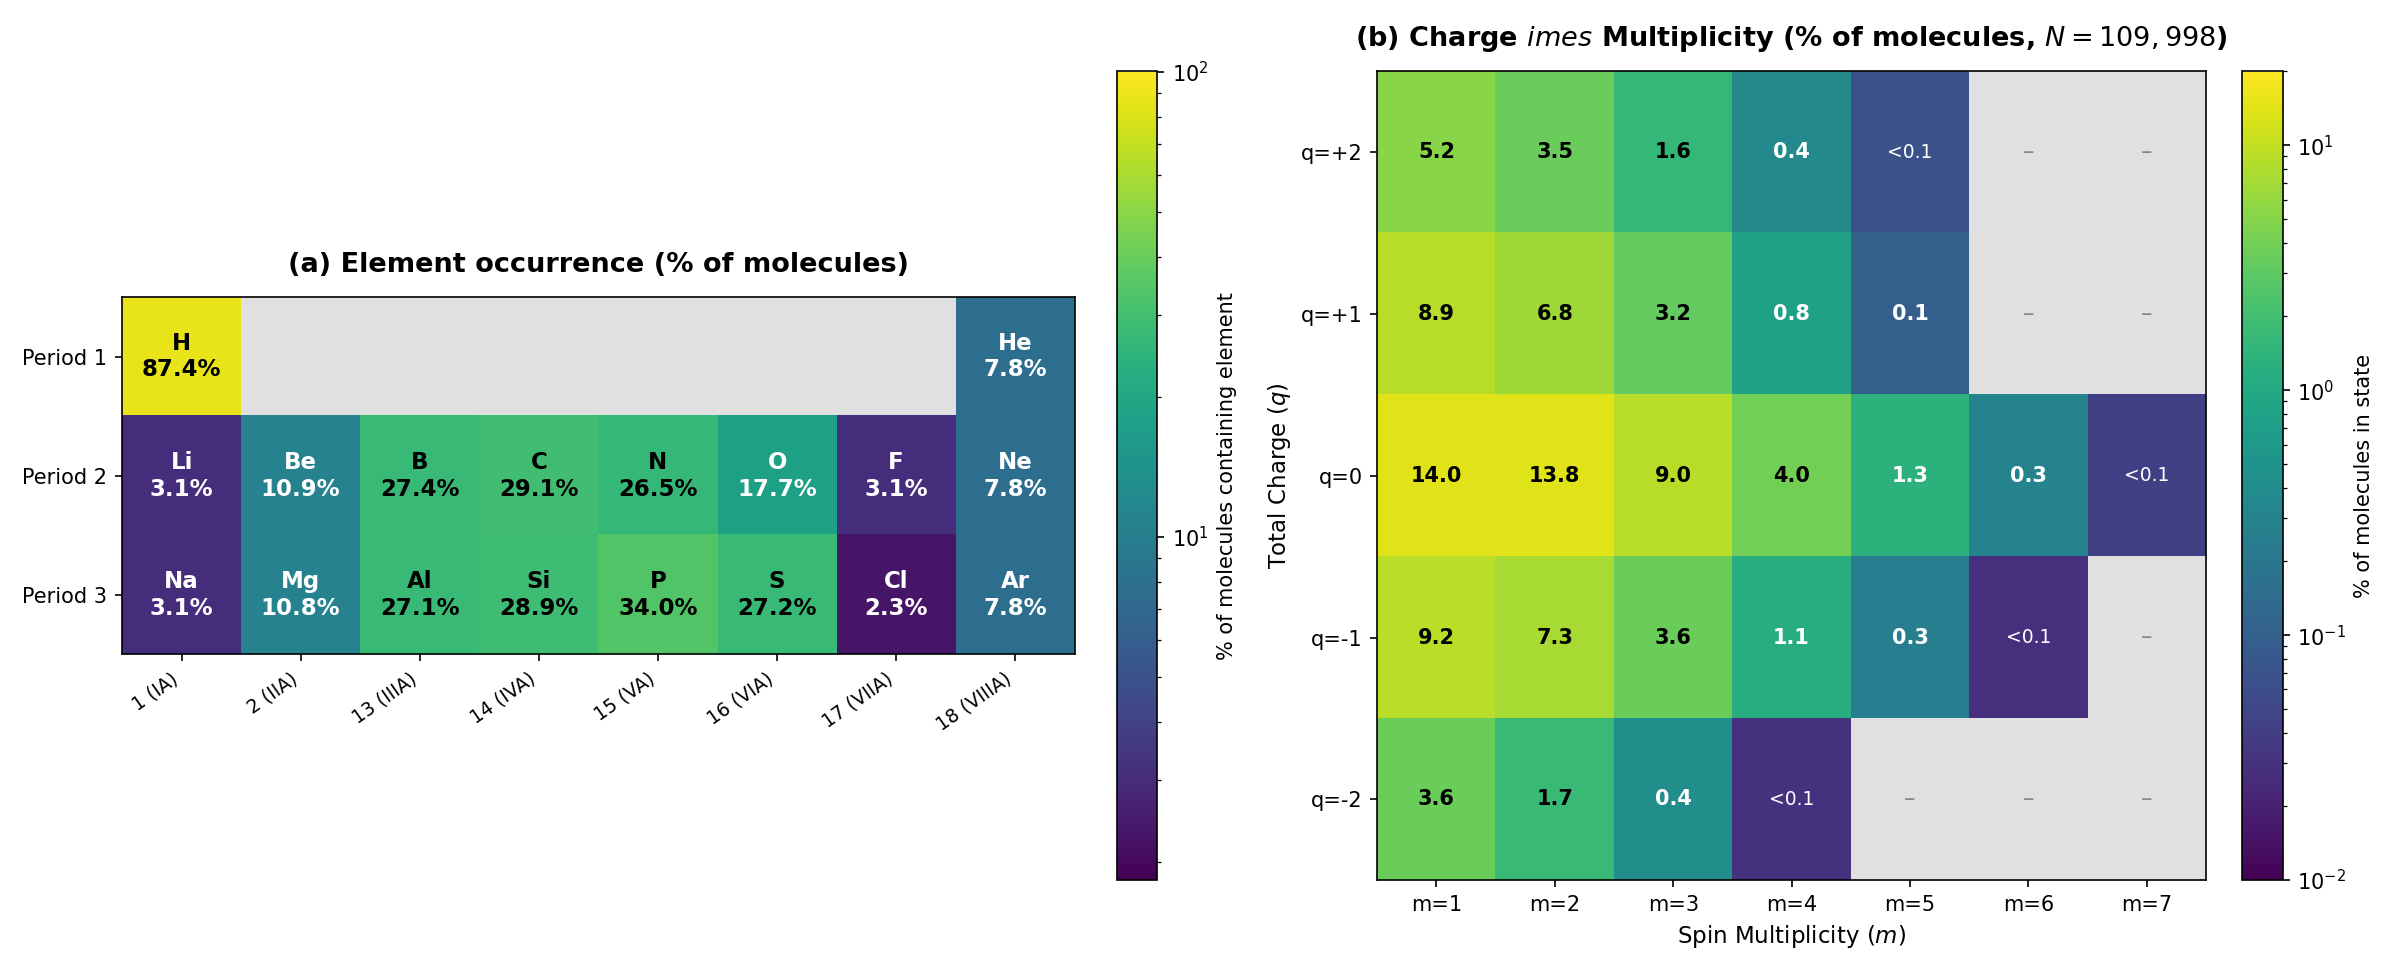
\includegraphics[width=0.95\textwidth]{task3_chemical_space_overview.png}
\caption{\textbf{Chemical space coverage of the 3-node subset ($N = 109{,}998$ molecules).} (a) Percentage of molecules containing at least one atom of the given element, arranged according to the periodic table (periods 1--3, groups 1, 2 and 13--18). All 18 elements from H to Ar occur in at least 2.3\% of the molecules. Percentages do not sum to 100\% because a molecule may contain several elements. (b) Distribution of molecules over total charge $Q$ (axis label $q$) and spin multiplicity $2S+1$ (axis label $m$); 26.1\% of the molecules have $2S+1 \ge 3$. Numbers in the cells are percentages of molecules; both colour scales are logarithmic. In (b), grey cells marked ``--'' denote charge--multiplicity combinations absent from the dataset, and ``$<$0.1'' marks non-zero fractions below 0.1\%.}
\label{fig:atom_distribution}
\end{figure}

\subsection*{Molecules with Multiple Calculations}

Some geometries have more than three QM calculations stored because multiple graph-level specifications (sharing the same total charge and spin multiplicity, such as resonance forms or alternative formal-charge and radical-site assignments) relaxed to identical 3D coordinates under UFF and had their distinct method/basis draws pooled. This occurs for 145 geometries (4.9\%, up to 3 specifications per geometry) in the 2-node subset and 6,134 geometries (5.6\%, up to 4 specifications per geometry) in the 3-node subset.

\section*{Technical Validation}

\subsection*{Bond Length Distributions}

Because nuclear coordinates were generated by 50-step UFF pre-relaxation rather than quantum-mechanical optimization, interatomic distances primarily reflect UFF covalent-radius parameterizations and serve here as a sanity check that pre-relaxation removes initial embedding distortions (Figure~\ref{fig:bond_lengths}). For representative covalent bonds involving period-2 elements (C--C, C--N, C--O), the distributions exhibit peaks centered near canonical UFF bond lengths (1.4--1.5~\AA{} for C--C, 1.3--1.4~\AA{} for C--N, and 1.2--1.4~\AA{} for C--O), spanning single- and multiple-bond regimes. Heteroatomic and less conventional pairs (such as Mg--Cl and Al--O) similarly exhibit unimodal distributions across non-equilibrium intervals.

\begin{figure}[ht!]
\centering
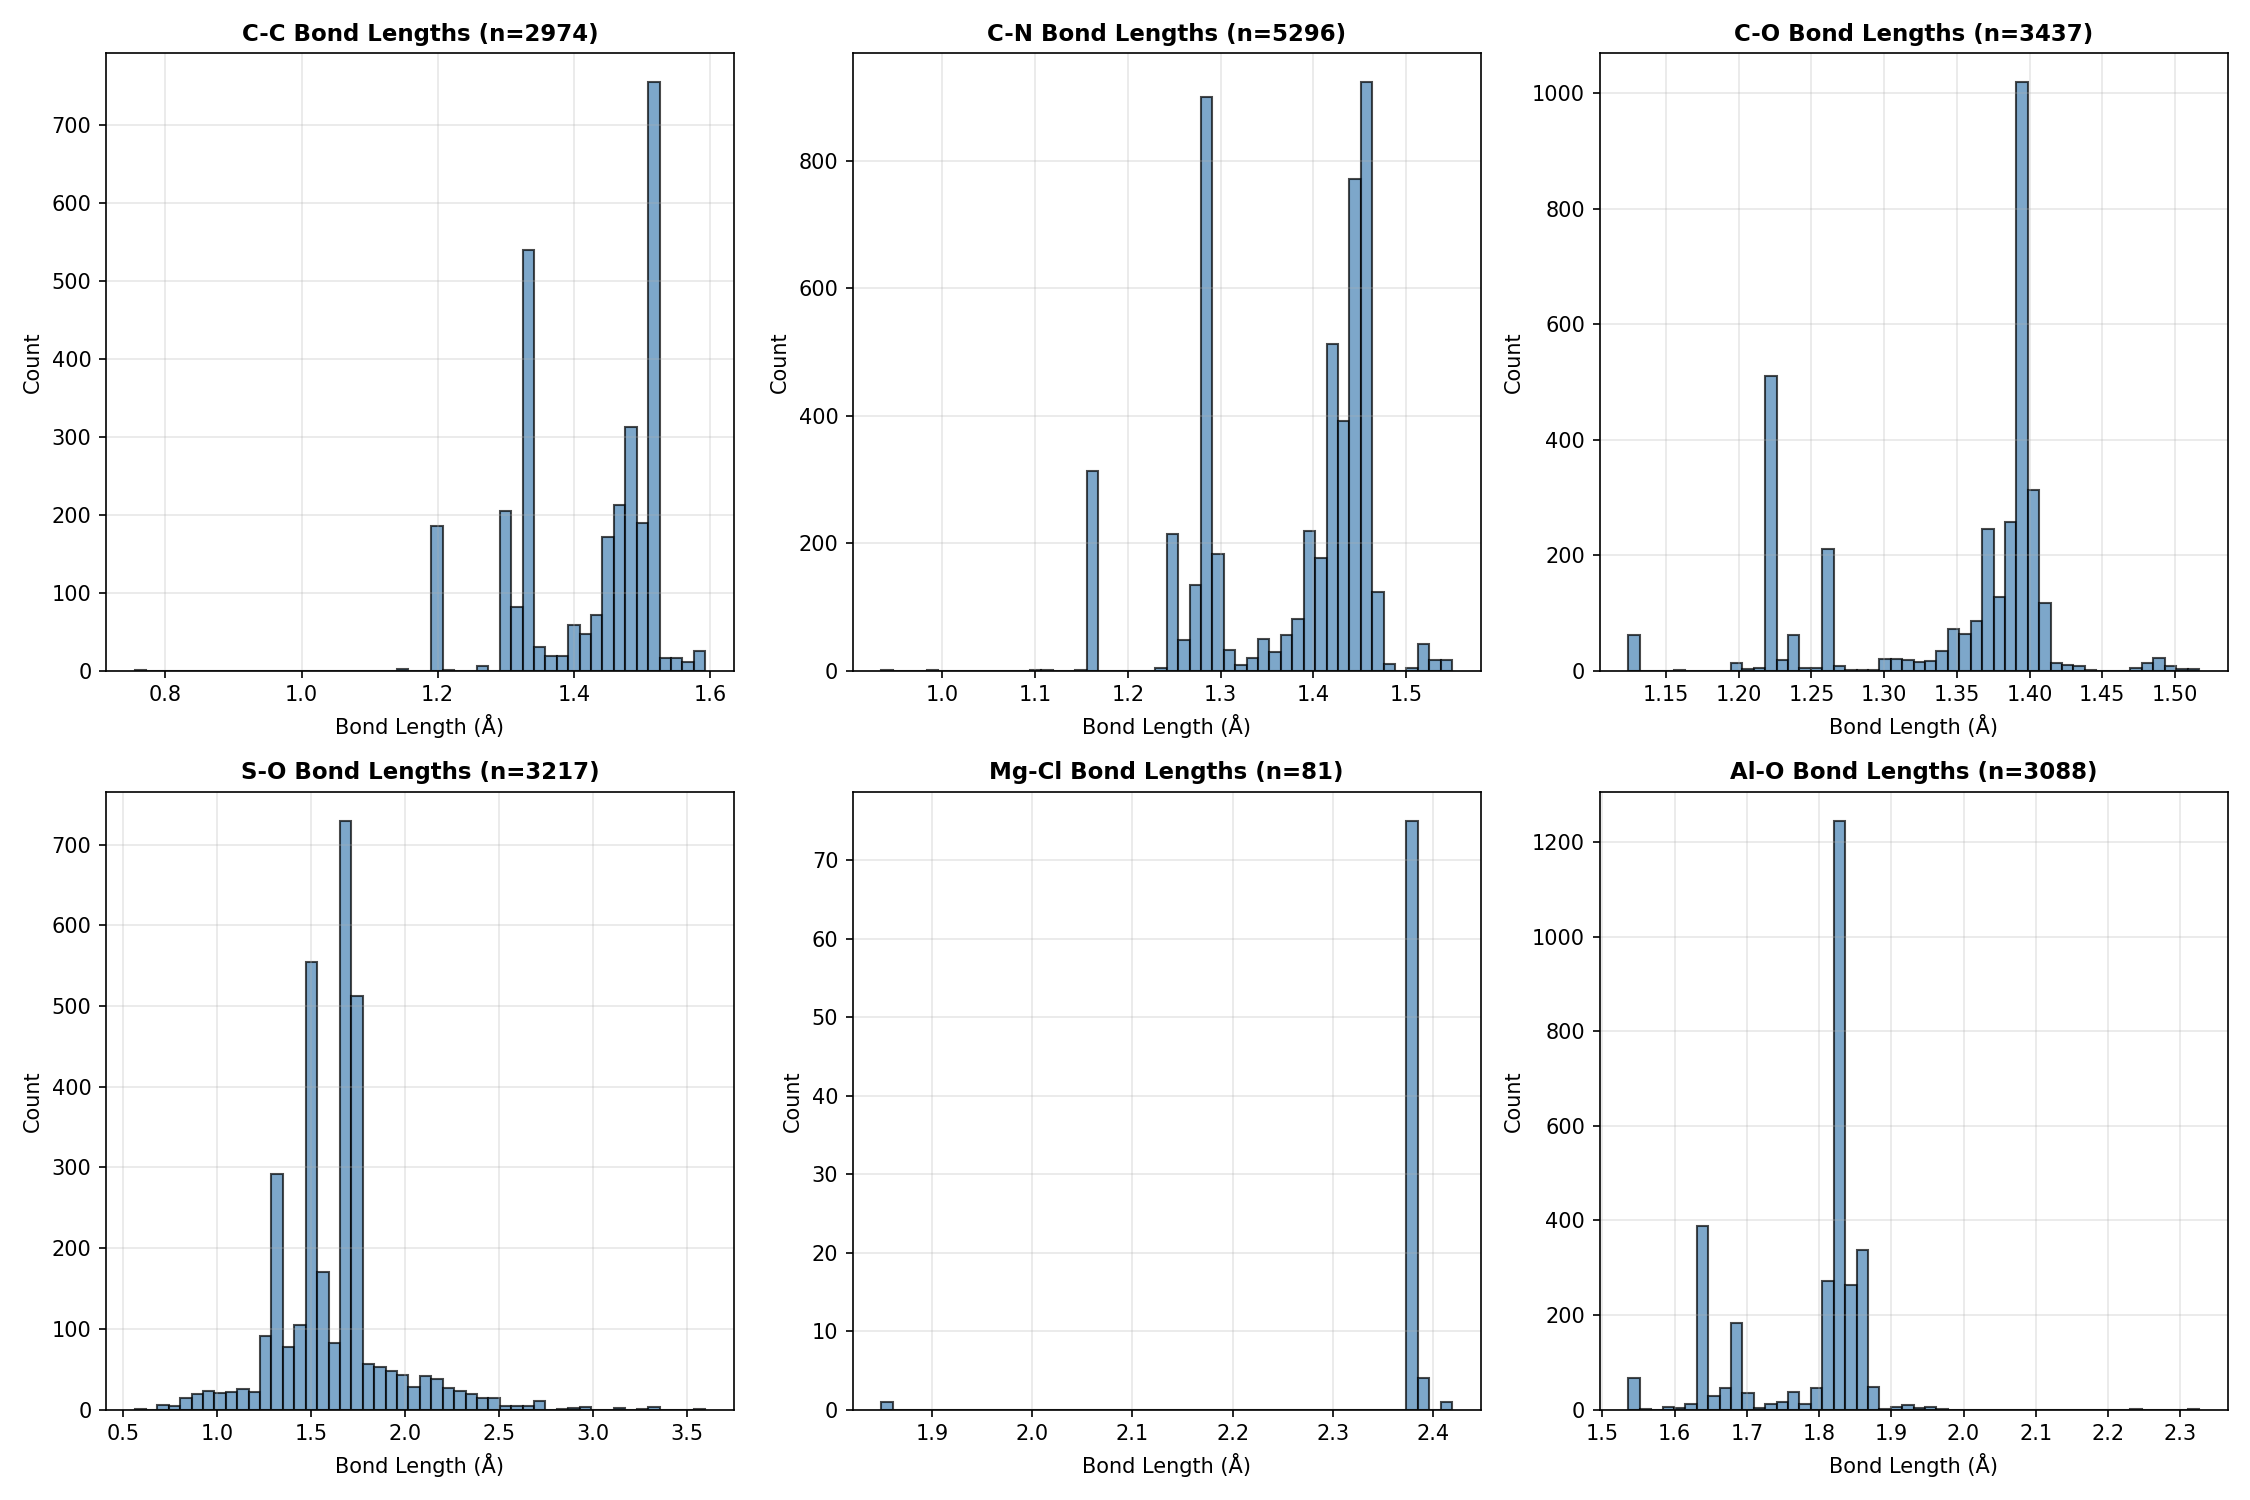
\includegraphics[width=0.9\textwidth]{task2_bond_length_histograms.png}
\caption{Bond length distributions for selected bonded atom pairs across the UFF pre-relaxed geometries. Distributions for organic linkages (C--C, C--N, C--O) cluster near standard covalent bond lengths, while heteroatomic pairings (Mg--Cl, Al--O) populate unimodal non-equilibrium intervals.}
\label{fig:bond_lengths}
\end{figure}

\subsection*{Periodic Trends in Bond Lengths}

Evaluation of half-bond lengths---defined here simply as half the interatomic distance ($r_{ij}/2$) across bonded atom pairs in the molecular graph---reproduces the expected periodic trends encoded in the force field. Figures~\ref{fig:half_bonds_C} and~\ref{fig:half_bonds_P} show the sawtooth variation of $r_{ij}/2$ as a function of the binding partner atomic number ($Z$). For carbon bonds (Figure~\ref{fig:half_bonds_C}), contracted separations occur for period-2 $p$-block partners (B, C, N, O, F) compared with period-3 partners (Na through Ar), consistent with periodic variations in covalent radii. Phosphorus (Figure~\ref{fig:half_bonds_P}) exhibits an analogous periodic profile shifted to larger separations, reflecting the larger covalent radius of a period-3 center. Together, these distributions confirm that the embedding and UFF pre-relaxation pipeline produces geometrically regular starting structures across periods 1--3 without systematic coordinate corruption.

\begin{figure}[ht!]
\centering
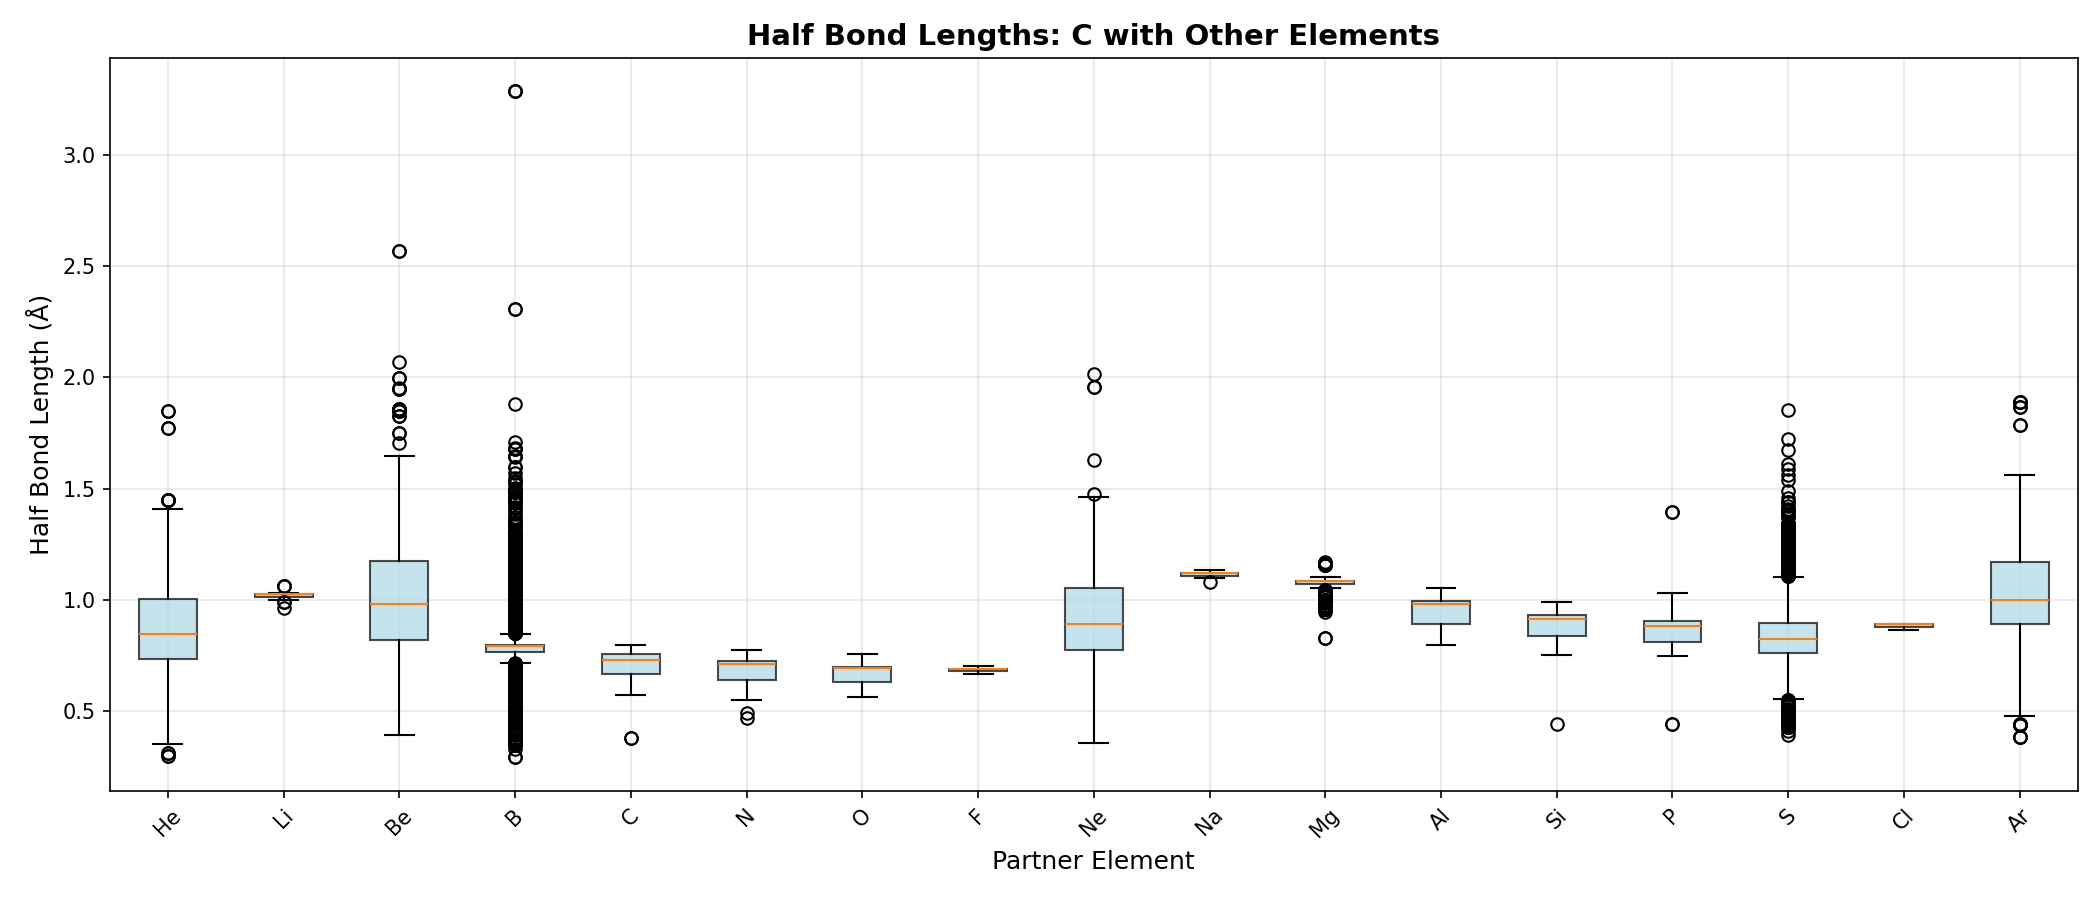
\includegraphics[width=0.9\textwidth]{task1_half_bonds_C.png}
\caption{Half-bond lengths ($r_{ij}/2$) for carbon across bonded partners ($Z=2$--$18$). The sawtooth profile reflects underlying covalent radii, with contracted separations for period-2 partners (B through F) and expanded distances for period-3 partners (Na through Ar). Box plots indicate quartiles and outliers across all evaluated C--X bonds.}
\label{fig:half_bonds_C}
\end{figure}

\begin{figure}[ht!]
\centering
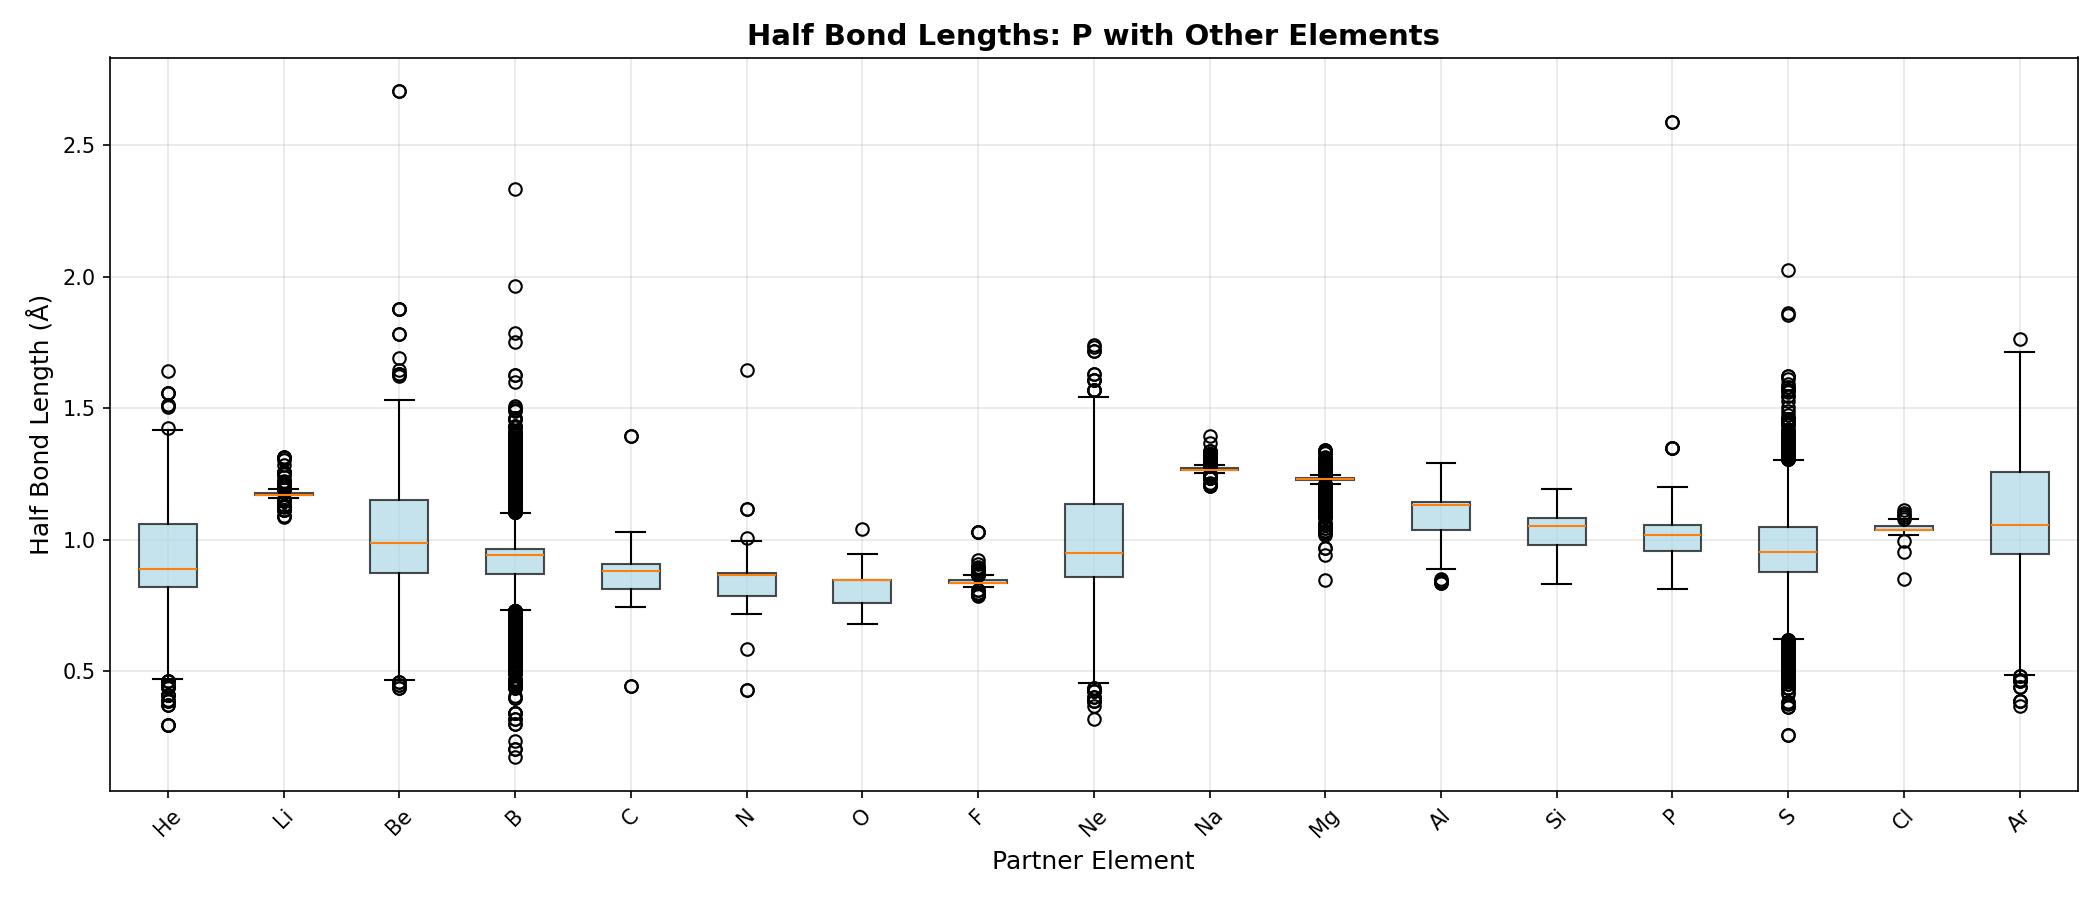
\includegraphics[width=0.9\textwidth]{task1_half_bonds_P.png}
\caption{Half-bond lengths ($r_{ij}/2$) for phosphorus across bonded partners ($Z=2$--$18$). The trend exhibits periodic modulation analogous to carbon, shifted toward larger interatomic distances in accordance with the larger covalent radius of period-3 phosphorus.}
\label{fig:half_bonds_P}
\end{figure}

\subsection*{SCF Energy Distributions}

All 338,616 released calculations (8,973 in the 2-node subset and 329,643 in the 3-node subset) terminated normally in Q-Chem and satisfied the $10^{-8}$~a.u.\ DIIS convergence criterion; for 2 geometries in the 2-node set (0.07\%) and 129 in the 3-node set (0.12\%), none of the assigned calculations converged and only \texttt{metadata.json} (\texttt{completeness = "0/3"}) is retained. Across all converged calculations, no positive SCF energies ($E_{\mathrm{SCF}} > 0$~Ha) or extreme negative outliers ($E_{\mathrm{SCF}} < -1{,}500$~Ha) occur. Total SCF energies span $-1{,}053.60$ to $-3.35$~Ha (median $-366.68$~Ha; $p_{1} = -867.02$~Ha, $p_{99} = -28.44$~Ha) in the 2-node subset and $-1{,}452.24$ to $-16.90$~Ha (median $-554.02$~Ha; $p_{1} = -1{,}169.34$~Ha, $p_{99} = -74.36$~Ha) in the 3-node subset (Figure~\ref{fig:energy_distributions}). Normalized per electron, $E_{\mathrm{SCF}}/N_e$ falls within $[-30.99, -1.67]$~Ha/$e^{-}$ (median $-15.81$~Ha/$e^{-}$) for 2-node and $[-29.03, -2.82]$~Ha/$e^{-}$ (median $-16.32$~Ha/$e^{-}$) for 3-node molecules, confirming consistent energy parsing and atomic-number assignments. Across the nine method--basis combinations, marginal distributions exhibit consistent ranges and multimodal bands governed by the discrete heavy-atom nuclear charges ($Z = 2$--$18$), with 3-node median energies ranging from $-558.05$~Ha ($\omega$B97X-D/DEF2-SVP) to $-547.03$~Ha ($\omega$B97X-D/STO-3G).

\begin{figure}[ht!]
\centering
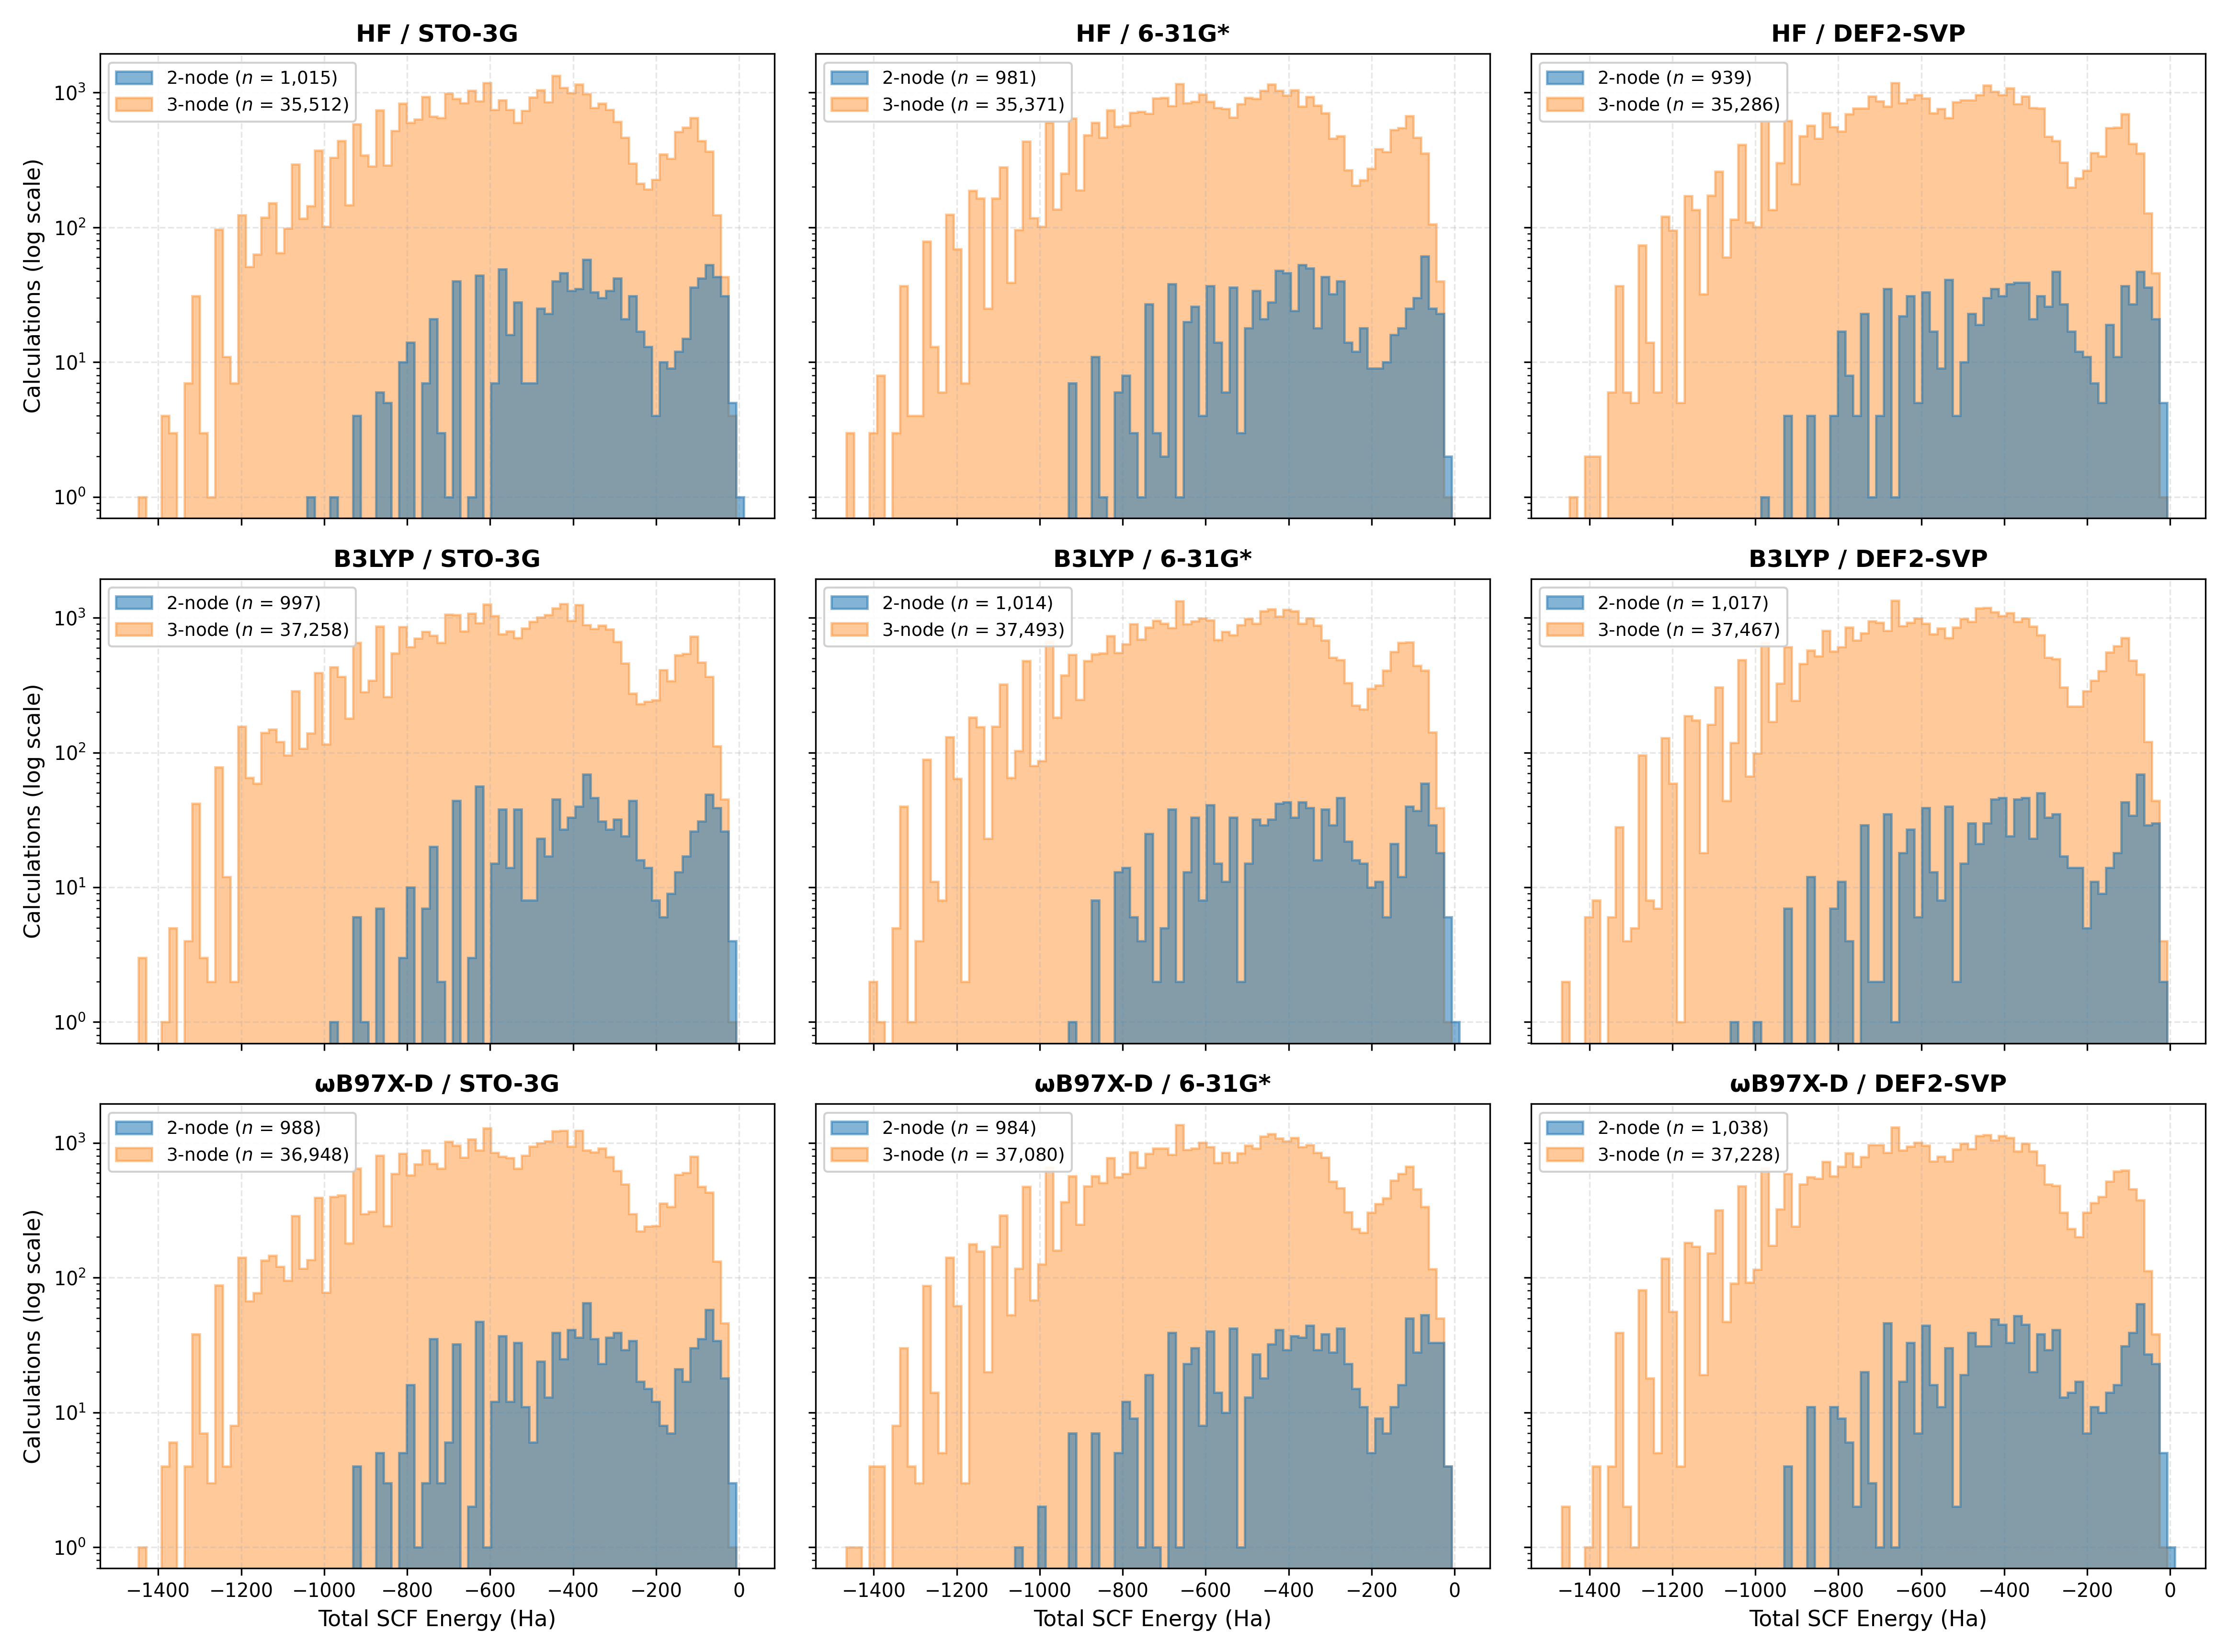
\includegraphics[width=0.95\textwidth]{energy_distributions_3x3.png}
\caption{Total SCF energy distributions across the nine method--basis combinations for the 2-node ($N = 8{,}973$ calculations, blue) and 3-node ($N = 329{,}643$ calculations, orange) subsets, shown with 80 equal-width bins on a logarithmic count scale. Multimodal structure reflects discrete heavy-atom compositions across periods 1--3; all converged energies are strictly negative.}
\label{fig:energy_distributions}
\end{figure}

\subsection*{Atomic Force Distributions and Electronic Method Consistency}

Because geometries were pre-relaxed with UFF under a constrained 50-iteration limit rather than converged to quantum-mechanical stationary points, atomic forces do not vanish identically but span a wide dynamic range ($10^{-5}$ to $>10^{2}$~Ha/Bohr, Figure~\ref{fig:forces}). Across the aggregate dataset ($N=35{,}804$ forces in the 2-node set and $N=1{,}766{,}211$ forces in the 3-node set), the median force magnitude is 0.0329~Ha/Bohr for 2-node molecules and 0.0379~Ha/Bohr for 3-node molecules (Table~\ref{tab:force_percentiles}). The 90th and 95th percentiles are 0.175~Ha/Bohr and 0.387~Ha/Bohr in the 2-node subset, and 0.233~Ha/Bohr and 0.550~Ha/Bohr in the 3-node subset, with higher values largely associated with the strongly compressed geometries discussed below.

\begin{figure}[ht!]
\centering
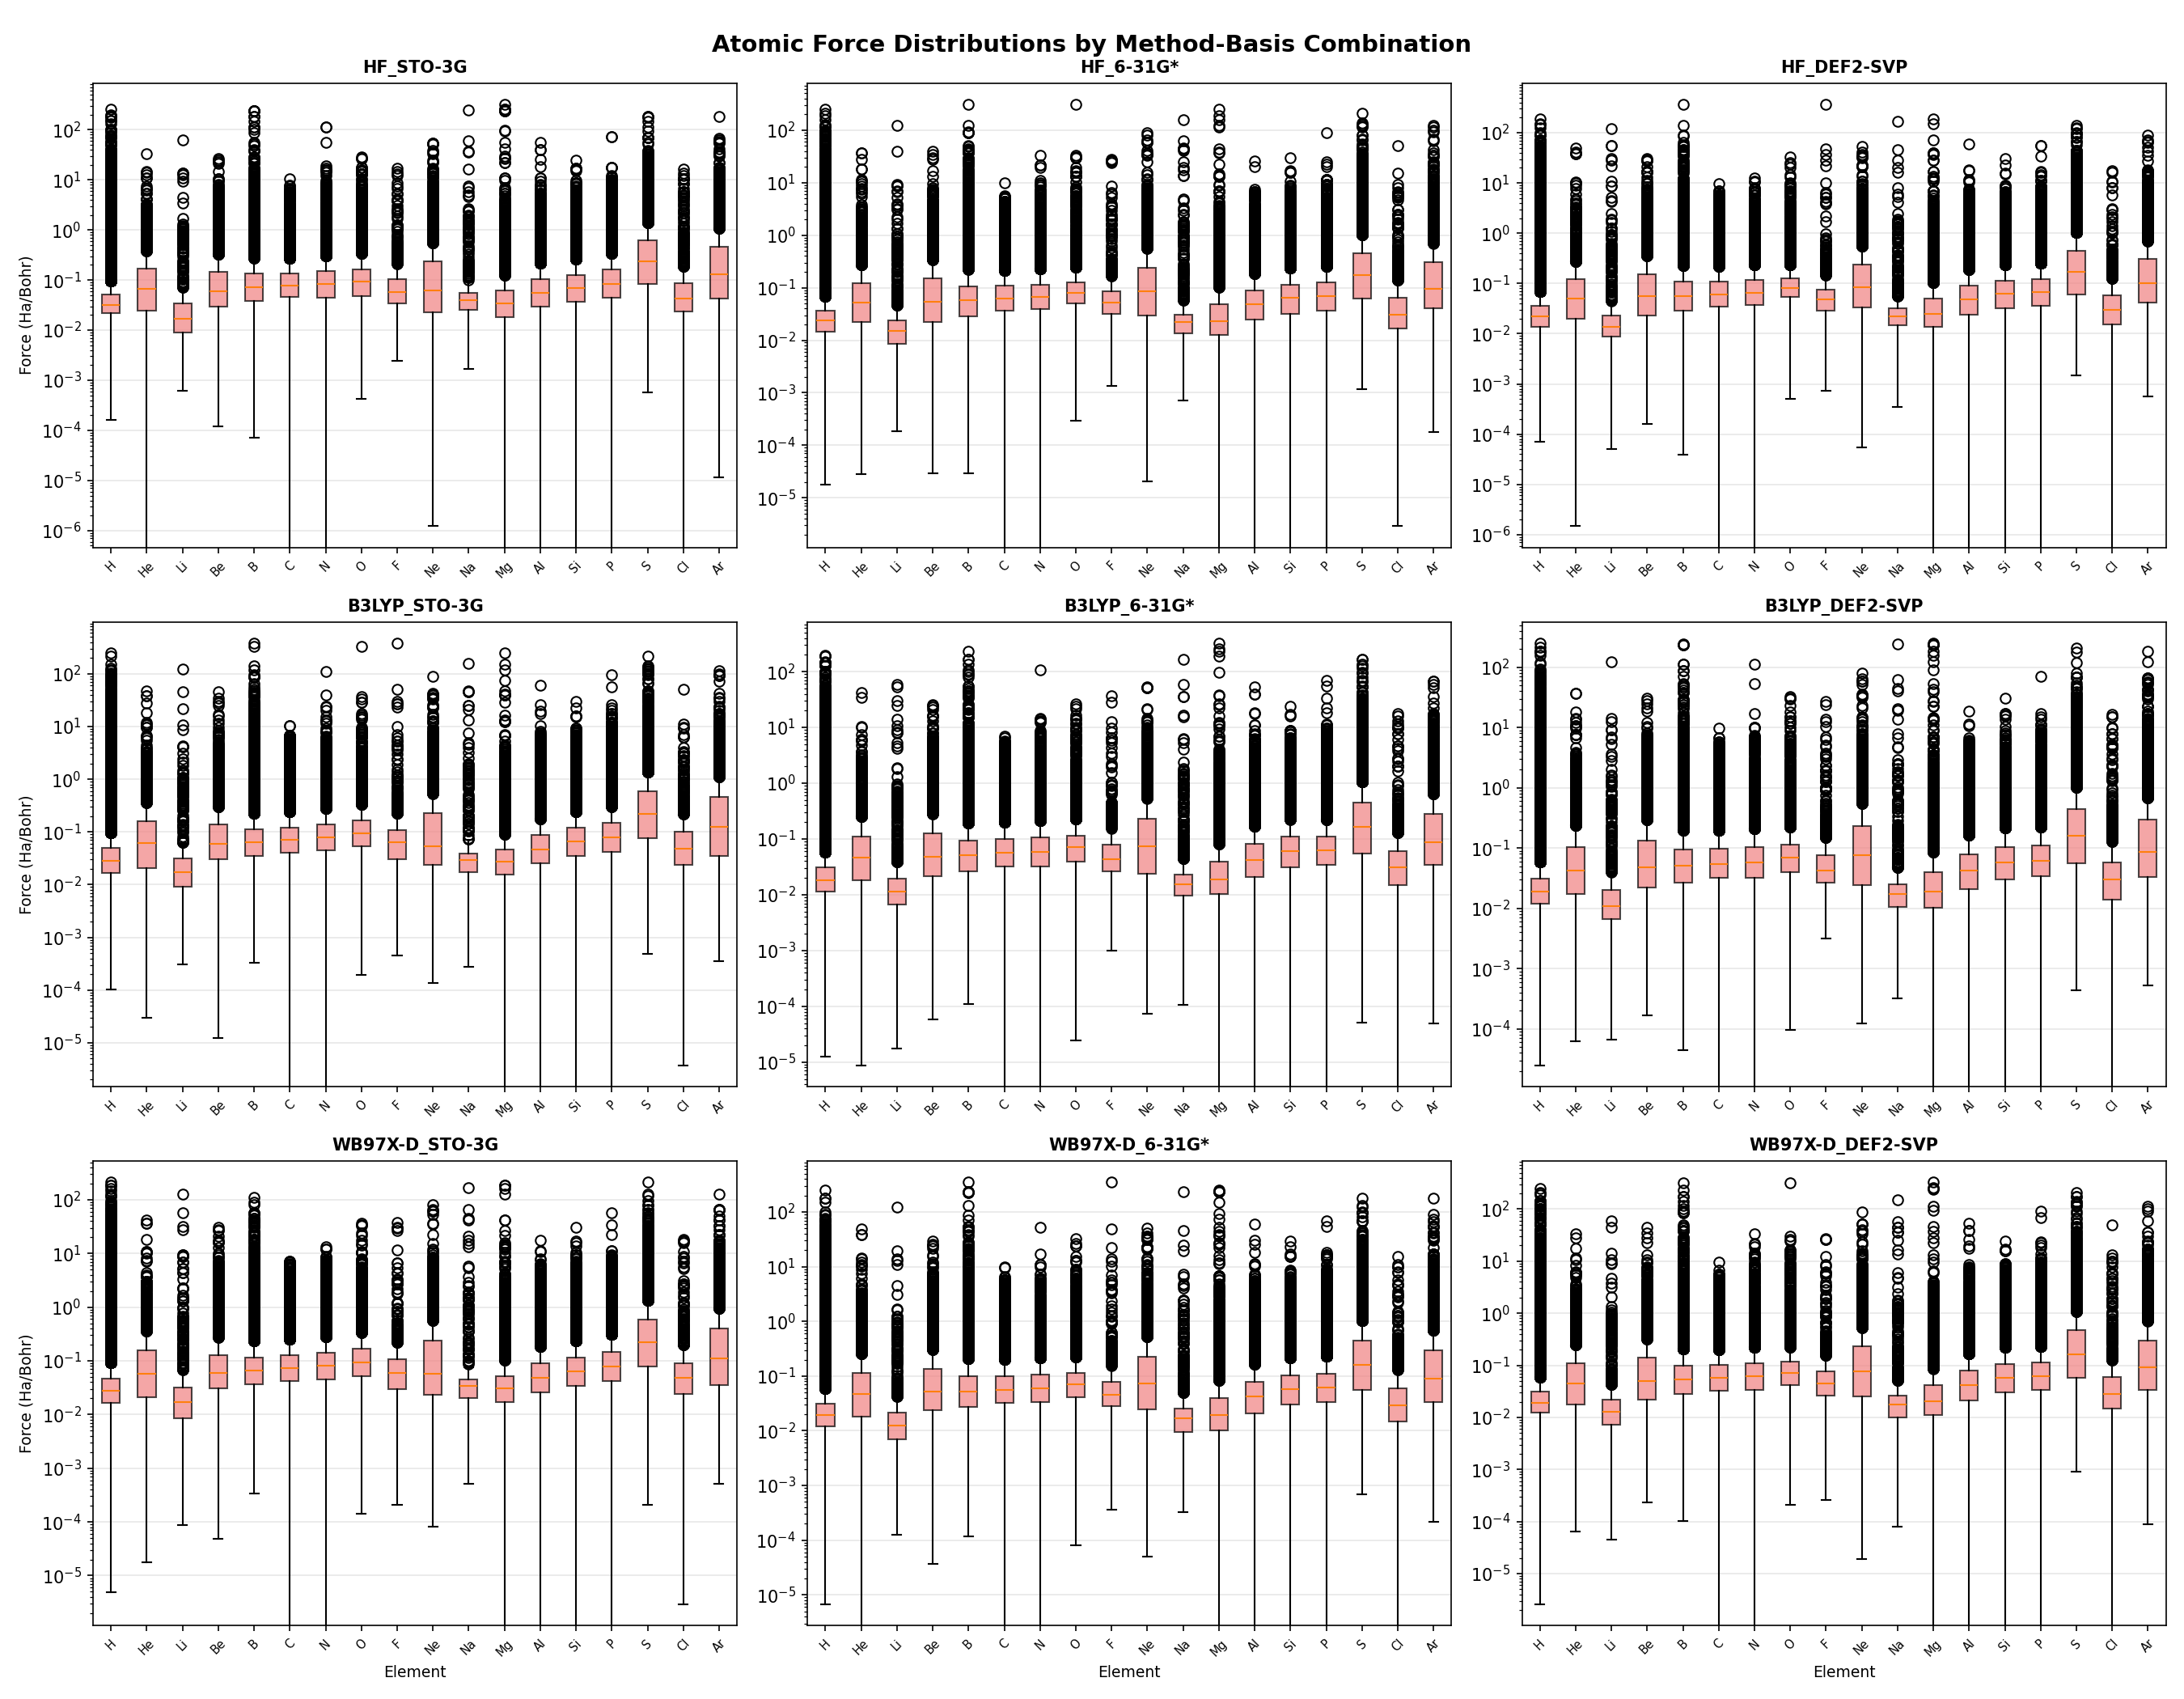
\includegraphics[width=0.9\textwidth]{task4_force_distribution.png}
\caption{Atomic force magnitude distributions by element across the 9 method--basis combinations. Log-scale distributions highlight that median force magnitudes remain clustered around $\sim$0.03--0.05~Ha/Bohr, with approximately 95\% of forces falling below 0.55~Ha/Bohr. The upper tail captures high-energy non-equilibrium configurations, including strongly compressed geometries in the predominantly repulsive regime.}
\label{fig:forces}
\end{figure}

Comparing marginal force distributions across the nine method--basis combinations (HF, B3LYP, and $\omega$B97X-D paired with STO-3G, 6-31G*, and DEF2-SVP; each combination evaluated on a pseudorandom one-third subset of specifications rather than all nine on every geometry) shows comparable overall force scales. In the 3-node dataset, median force magnitudes across the nine combinations fall within 0.0320--0.0480~Ha/Bohr, and the 99th percentiles fall within 3.87--4.25~Ha/Bohr, indicating that aggregate force scales are governed primarily by the pre-relaxed nuclear geometries rather than method- or basis-specific outliers.

\begin{table}[ht!]
\centering
\begin{tabular}{lrrrrrr}
\toprule
Subset & Median ($p_{50}$) & $p_{75}$ & $p_{90}$ & $p_{95}$ & $p_{99}$ & $p_{99.9}$ \\
\midrule
2-node aggregate ($N=35{,}804$) & 0.0329 & 0.0699 & 0.1745 & 0.3867 & 1.9154 & 18.7990 \\
3-node aggregate ($N=1{,}766{,}211$) & 0.0379 & 0.0912 & 0.2329 & 0.5498 & 4.0387 & 24.5763 \\
\bottomrule
\end{tabular}
\caption{Aggregate atomic force magnitude percentiles (in Ha/Bohr) for 2-node and 3-node molecular sets across all nine quantum-chemical calculations (3 basis sets, 3 methods).}
\label{tab:force_percentiles}
\end{table}

\subsection*{Geometric Crowding and Short-Range Repulsive Regime}

To rigorously characterize structures exhibiting elevated forces without relying on calculation-specific metrics, we performed coordinate-based geometry analyses across all unique molecular configurations. In small-molecule combinatorial enumeration (2--3 heavy atoms), unconstrained valence saturation and empirical force-field limitations occasionally produce sterically crowded configurations. Using a covalent-radius normalized distance ratio ($r_{ij} / r_{\text{cov}}$), configurations were classified into three geometric regimes (Table~\ref{tab:crowding_stats}):
\begin{enumerate}
\item \textbf{Uncrowded geometries (\texttt{none}):} Comprising 98.92\% of the 2-node set (2,926 molecules) and 96.80\% of the 3-node set (106,355 molecules), where all interatomic distances satisfy $r_{ij} / r_{\text{cov}} \ge 0.50$.
\item \textbf{Isolated crowded pairs (\texttt{clean\_pair}):} 0.85\% of 2-node (25 molecules) and 2.74\% of 3-node (3,012 molecules), featuring an isolated compressed contact ($r_{ij} / r_{\text{cov}} < 0.50$, median minimum distance 0.37~\AA{}) while maintaining otherwise unperturbed molecular topology.
\item \textbf{Crowded clusters (\texttt{crowded\_cluster}):} 0.24\% of 2-node (7 molecules) and 0.46\% of 3-node (502 molecules), where multiple compressed contacts occur simultaneously (e.g., multi-hydrogen crowding around over-coordinated sulfur or coordination-deficient boron/beryllium centers).
\end{enumerate}

\begin{table}[ht!]
\centering
\begin{tabular}{lrrrr}
\toprule
Geometric Category & 2-node Count & 2-node \% & 3-node Count & 3-node \% \\
\midrule
Uncrowded (\texttt{none}) & 2,926 & 98.92\% & 106,355 & 96.80\% \\
Isolated pair crowding (\texttt{clean\_pair}) & 25 & 0.85\% & 3,012 & 2.74\% \\
Cluster crowding (\texttt{crowded\_cluster}) & 7 & 0.24\% & 502 & 0.46\% \\
\midrule
Total unique geometries & 2,958 & 100.00\% & 109,869 & 100.00\% \\
\bottomrule
\end{tabular}
\caption{Classification of unique molecular geometries based on normalized interatomic distance ratios ($r_{ij} / r_{\text{cov}}$). Evaluated across all geometries with at least one converged quantum chemical calculation (excluding the 2 and 129 geometries in the 2-node and 3-node subsets, respectively, for which no SCF calculations converged).}
\label{tab:crowding_stats}
\end{table}

Direct cross-referencing between geometric outliers and quantum-mechanical force magnitudes indicates that extreme atomic forces ($>10$~Ha/Bohr) are predominantly associated with very close nuclear encounters. In the 2-node dataset, only 8 unique molecules (0.27\% of converged geometries; 24 calculations, 0.27\% of calculations) exhibit forces $>10$~Ha/Bohr, having a median minimum distance of 0.143~\AA{}. In the 3-node dataset, 1,046 unique molecules (0.95\% of converged geometries; 2,942 calculations, 0.89\% of calculations) meet this criterion, with a median minimum interatomic distance of 0.249~\AA{} (1,045 of the 1,046 geometries satisfy $r_{ij}/r_{\mathrm{cov}} < 0.50$, including 47 heavy-atom short contacts with $d_{\min} \in [0.80, 0.96]$~\AA{}). Conversely, a distinct subset of compressed geometries with $d_{\min} < 0.50$~\AA{} (17 converged geometries in 2-node and 1,255 in 3-node; median $d_{\min} \approx 0.37$~\AA{}) maintains moderate forces $\le 10$~Ha/Bohr.

Two-body radial force and sign-alignment evaluations ($f_{\mathrm{rel}} = \frac{1}{2}(\mathbf{F}_i - \mathbf{F}_j)\cdot\hat{\mathbf{r}}_{ij}$, with $\hat{\mathbf{r}}_{ij}$ pointing from atom $j$ to atom $i$) confirm that compressed nearest-neighbor configurations are predominantly repulsive across polyatomic molecules ($N_{\mathrm{atoms}} \ge 3$): for atom-centered nearest-neighbor entries pooled across all calculations, $f_{\mathrm{rel}} > 0$ holds for 97.0\% below 0.8~\AA{} ($n = 867$) and 100.0\% below 0.5~\AA{} ($n = 187$) in the 2-node subset, and for 94.3\% below 0.8~\AA{} ($n = 47{,}132$) and 97.2\% below 0.5~\AA{} ($n = 14{,}972$) in the 3-node subset. Across the compressed regime ($r_{ij}/r_{\mathrm{cov}} < 0.9$), binned median $|f_{\mathrm{rel}}|$ magnitudes increase steadily with decreasing compression ratio, without abrupt discontinuities or numerical collapse. In all released calculations, the SCF procedure achieved electronic convergence ($10^{-8}$~a.u.), so that the reported values represent analytic forces (negative energy gradients) of the converged SCF energy.

For applications that should exclude strongly compressed contacts, structures can be filtered with the coordinate-based criterion $r_{ij} / r_{\text{cov}} \ge 0.50$ for all atom pairs, which retains 98.9\% (2-node) and 96.8\% (3-node) of the analyzed geometries. The excluded configurations (Table~\ref{tab:crowding_stats}) can instead serve as test cases for the short-range repulsive behavior of interatomic potentials.

\subsection*{Archive Integrity and Matrix Identities}

Automated single-pass validation across all 112,958 molecule directories and 338,616 \texttt{.npz}/\texttt{.qcout} calculation pairs confirmed zero missing or corrupted files, zero \texttt{NaN}/\texttt{Inf} array entries, zero intra- or inter-subset \texttt{geometry\_\allowbreak{}hash} collisions, and zero violations of the single-specification Latin-square method/basis assignment. Pairwise interatomic distances reconstructed from \texttt{.npz} standard-orientation coordinates (in Bohr) match those from input-orientation coordinates in \texttt{metadata.json} within $5.26 \times 10^{-6}$~\AA{} (2-node) and $7.32 \times 10^{-6}$~\AA{} (3-node), and standard-orientation coordinates agree within $10^{-4}$~\AA{} across all multi-calculation geometries. Core Hamiltonian additivity ($\|T + V - H_{\mathrm{core}}\|_{\max} \le 3.05 \times 10^{-5}$~a.u.) and translational force invariance ($\|\sum_i \mathbf{F}_i\| \le 1.76 \times 10^{-5}$~Ha/Bohr) hold to \texttt{float32} precision across both subsets.

For the electronic-structure matrices, electron-count normalization $|\mathrm{Tr}(P_{\mathrm{tot}} S) - N_e|$ has a median residual of $1.32 \times 10^{-7}$ (maximum $7.81 \times 10^{-6}$) in the 2-node subset and $1.62 \times 10^{-7}$ ($p_{99} = 9.54 \times 10^{-7}$, maximum $2.68 \times 10^{-4}$, exceeding $10^{-4}$ in 8 calculations) in the 3-node subset, while open-shell spin-density normalization $|\mathrm{Tr}(P_{\mathrm{spin}} S) - (N_\alpha - N_\beta)|$ holds within $4.22 \times 10^{-5}$ across all 199,926 open-shell calculations. Molecular orbital orthonormality $\|C S C^{\top} - I_{N_{\mathrm{indep}}}\|_{\max}$ has a median residual of $9.54 \times 10^{-7}$ (maximum $1.43 \times 10^{-4}$, 1 calculation $>10^{-4}$) in 2-node and $1.41 \times 10^{-6}$ ($p_{99} = 1.96 \times 10^{-5}$, maximum $4.86 \times 10^{-3}$, exceeding $10^{-4}$ in 168 calculations and $10^{-3}$ in 17 calculations) in 3-node; the largest residuals occur in \texttt{float32} storage when compressed interatomic contacts render $S$ nearly singular. Across the entire dataset, AO near-linear dependence ($N_{\mathrm{indep}} < N_{\mathrm{bas}}$) occurs in a single calculation (\texttt{dataset\_\allowbreak{}3node/mol\_\allowbreak{}086465}, $\omega$B97X-D/DEF2-SVP, $d_{\min} = 0.1014$~\AA{}, $N_{\mathrm{bas}} = 89$, $N_{\mathrm{indep}} = 88$). Reconstructing $P_{\mathrm{tot}}$ from the occupied MO rows ($2 C_{\mathrm{occ}}^{\top} C_{\mathrm{occ}}$ for closed-shell and $C_{\mathrm{occ},\alpha}^{\top} C_{\mathrm{occ},\alpha} + C_{\mathrm{occ},\beta}^{\top} C_{\mathrm{occ},\beta}$ for open-shell systems) matches the stored SCF density within $4.73 \times 10^{-6}$ (2-node) and $1.42 \times 10^{-4}$ (3-node).

\subsection*{Frontier Orbital Sign and Open-Shell Spin Contamination}

Because the three basis sets (STO-3G, 6-31G*, and DEF2-SVP) omit diffuse functions to keep the AO representation compact across 18 elements, gas-phase anions ($Q < 0$) frequently exhibit positive highest occupied molecular orbital eigenvalues ($\varepsilon_{\mathrm{HOMO}} > 0$, taking $\max(\varepsilon_{\mathrm{HOMO},\alpha}, \varepsilon_{\mathrm{HOMO},\beta})$ for open-shell states). Specifically, $\varepsilon_{\mathrm{HOMO}} > 0$ occurs in 79.9\% (2,651/3,319) of 2-node and 70.3\% (64,565/91,879) of 3-node anionic calculations---including 100.0\% of dianions ($Q=-2$) in both subsets and 70.5\% (2-node) and 62.3\% (3-node) of monoanions ($Q=-1$)---compared with 5.2\% and 5.7\% for neutral species ($Q=0$) and 0.0\% for cations ($Q>0$). Within the 3-node anionic subset, positive HOMO fractions are near unity in minimal STO-3G bases (99.2--100.0\%) and in B3LYP split-valence calculations (93.5\% in 6-31G*, 92.9\% in DEF2-SVP), whereas Hartree--Fock (34.5\% in 6-31G*, 33.2\% in DEF2-SVP) and range-separated $\omega$B97X-D (39.3\% and 36.9\%) bind a substantially larger fraction of monoanions. Users targeting electron detachment energies or asymptotic anion densities should account for this basis-set limitation.

All open-shell calculations (4,733 in 2-node and 195,193 in 3-node) employed unrestricted formalisms (UHF or UKS). Spin contamination $\Delta\langle S^2\rangle = \langle S^2\rangle - S(S+1)$ parsed from the \texttt{.qcout} files has a median of $0.0070$ ($p_{95} = 0.170$, maximum $1.073$) in the 2-node subset, with $|\Delta\langle S^2\rangle| > 0.1$ in 7.8\% of open-shell runs (14.2\% for UHF versus 4.8\% for UKS) and $> 0.5$ in 1.0\%. In the 3-node subset, $\Delta\langle S^2\rangle$ has a median of $0.0174$ ($p_{95} = 0.403$, maximum $2.103$), exceeding $0.1$ in 17.6\% of open-shell runs (30.8\% for UHF versus 11.5\% for UKS) and $0.5$ in 3.6\% (6.0\% for UHF versus 2.4\% for UKS). Applications requiring spin-pure open-shell references can filter directly on $\langle S^2\rangle$ parsed from the \texttt{.qcout} files.

\section*{Usage Notes}

\subsection*{Loading the Data}

Example Python code to load coordinates, forces, AO matrices, MO coefficients, and total energy:

\begin{verbatim}
import json
import numpy as np

def unpack_tril(vec, n):
    """Unpack a 1D lower-triangular vector into a symmetric (n, n) matrix."""
    mat = np.zeros((n, n), dtype=vec.dtype)
    mat[np.tril_indices(n)] = vec
    return mat + mat.T - np.diag(np.diag(mat))

mol_dir = 'dataset_2node/mol_000005'
with open(f'{mol_dir}/metadata.json') as f:
    metadata = json.load(f)

rep = metadata['representative_structure']
charge, mult = rep['total_charge'], rep['multiplicity']

# Pick the first available calculation from metadata
calc_name, calc_info = next(iter(metadata['available_calculations'].items()))
data = np.load(f"{mol_dir}/{calc_info['npz_file']}")

n_atoms = int(data['step_0_number_of_atoms'])
coords = data['step_0_current_cartesian_coordinates'].reshape(n_atoms, 3)  # Bohr
forces = data['step_0_cartesian_forces'].reshape(n_atoms, 3)              # Ha/Bohr

n_bas = int(data['step_0_number_of_basis_functions'])
n_indep = int(data['step_0_number_of_independent_functions'])
S = unpack_tril(data['step_0_overlap_matrix'], n_bas)
P_tot = unpack_tril(data['step_0_total_scf_density'], n_bas)
# Rows are MOs, columns are AOs (transpose for column-MO convention)
C_alpha = data['step_0_alpha_mo_coefficients'].reshape(n_indep, n_bas)
# float32 storage: up to ~5e-3 MO ortho drift at compressed contacts
assert np.allclose(C_alpha @ S @ C_alpha.T, np.eye(n_indep), atol=1e-2)
n_elec = int(data['step_0_number_of_electrons'])
assert np.isclose(np.trace(P_tot @ S), n_elec, atol=1e-3)

# Open-shell calculations also store beta MOs and spin density
if 'step_0_beta_mo_coefficients' in data:
    C_beta = data['step_0_beta_mo_coefficients'].reshape(n_indep, n_bas)
    P_spin = unpack_tril(data['step_0_spin_scf_density'], n_bas)

# Energy must be parsed from .qcout
with open(f"{mol_dir}/{calc_info['qcout_file']}") as f:
    for line in f:
        if 'SCF   energy in the final basis set' in line:
            total_energy = float(line.split('=')[1].strip())
            break
\end{verbatim}

\subsection*{Working with Alternative Structures}

For geometries shared by several specifications, the \texttt{metadata.json} file lists all of them under \texttt{alternative\_\allowbreak{}structures\_\allowbreak{}details}. The total charge and multiplicity of each specification follow from its atomic states, $Q=\sum_i q_i$ and $2S+1=\sum_i n_{r,i}+1$. In the released dataset, all specifications sharing a geometry have the same $Q$ and $2S+1$ (verified against the charge and multiplicity of the corresponding Q-Chem inputs), i.e.\ they pose the same electronic structure problem and differ only in their Lewis-structure label. The calculations listed under \texttt{available\_\allowbreak{}calculations} are therefore valid for all specifications of a geometry. Machine learning models operating on molecular graphs should treat such specifications as distinct inputs with identical targets.

\begin{verbatim}
from collections import defaultdict

if metadata['num_alternative_structures'] > 1:
    groups = defaultdict(list)
    for spec in metadata['alternative_structures_details']:
        states = spec['atom_states'].values()
        q = sum(s['charge'] for s in states)
        # high-spin convention: all unpaired electrons are parallel
        mult = sum(s['unpaired_electrons'] for s in states) + 1
        groups[(q, mult)].append(spec['smiles'])

    for (q, mult), smiles in groups.items():
        print(f'Q={q:+d}, 2S+1={mult}: {smiles}')

# Note: atom_states cover heavy atoms only (hydrogens are implicit).
# In this dataset hydrogens carry no formal charge or unpaired electron,
# so the sums above give the total charge and multiplicity.
\end{verbatim}

%------------------------------------------------------------
\subsection*{Filtering Guidelines for Machine Learning}

Depending on the intended machine learning application, users can partition the dataset into low-strain and high-strain regimes using geometric and force criteria. Here, \emph{low-strain} denotes calculations satisfying both criteria below and \emph{high-strain} all remaining ones; the terms are used operationally, not in the sense of a computed strain energy:

\begin{verbatim}
import numpy as np
from scipy.spatial.distance import pdist

# Load coordinates and forces from parsed NPZ archive
# note coords in npz are in standard orientation and in Bohr
data = np.load('dataset_3node/mol_000001/B3LYP_6-31G*.npz')
n_atoms = int(data['step_0_number_of_atoms'])
coords_bohr = data['step_0_current_cartesian_coordinates'].reshape(n_atoms, 3)
coords = coords_bohr * 0.529177210903  # Bohr to Angstrom
forces = data['step_0_cartesian_forces'].reshape(n_atoms, 3)


min_dist = np.min(pdist(coords))
max_force = np.max(np.linalg.norm(forces, axis=1))

# Low-strain criterion (d_min >= 0.60 Angstrom and F_max <= 1.0 Ha/Bohr):
is_low_strain = (min_dist >= 0.60) and (max_force <= 1.0)
\end{verbatim}

To obtain a low-strain training set for neural network potentials, applying both criteria ($d_{\min} \geq 0.60$~\AA{} and $\|\mathbf{F}\|_{\max} \leq 1.0$~Hartree/Bohr) retains 95.8\% (2-node) and 92.3\% (3-node) of the individual calculations. Requiring a geometry to pass in all of its converged calculations retains 95.2\% and 91.7\% of the geometries, respectively (geometries without any converged calculation excluded). The force criterion alone is satisfied by 97.6\% and 96.7\% of all per-atom force vectors, pooled over all calculations. The coordinate-based criterion $r_{ij}/r_{\mathrm{cov}} \geq 0.50$ discussed above is a looser, purely geometric filter (Table~\ref{tab:crowding_stats}): among converged geometries, both filters pass simultaneously for 95.2\% of 2-node (2,816/2,958; 0 passing low-strain only) and 91.7\% of 3-node structures (100,754/109,869; only 25 passing low-strain while flagged by $r_{ij}/r_{\mathrm{cov}} < 0.50$, corresponding to compressed heavy-atom pairs with $d_{\min} \geq 0.60$~\AA{} and $\|\mathbf{F}\|_{\max} \leq 1.0$~Ha/Bohr).
Conversely, the high-strain remainder (or the complete unfiltered dataset) provides test cases for short-range repulsive interactions.

\section*{Data Availability}

The complete dataset is available on Zenodo\cite{zenodo_doi} under a Creative Commons Attribution 4.0 International (CC BY 4.0) license. The dataset includes two main compressed archives: \texttt{dataset\_2node.tar.gz} containing 2,960 molecules with 8,973 calculations, and \texttt{dataset\_3node.tar.gz} containing 109,998 molecules with 329,643 calculations. Each molecule directory contains metadata.json files, Q-Chem output files (.qcout), and parsed data in NumPy format (.npz).

\section*{Code Availability}
The validation and analysis scripts used to verify archive integrity, characterize geometric crowding, and generate the validation statistics and figures reported here (including \texttt{verify\_datasets.py}, \texttt{analyze\_dataset.py}, \texttt{crowding\_detector.py}, \texttt{sign\_alignment\_check.py}, \texttt{nn\_force\_distance\_v2.py}, and \texttt{ratio\_vs\_force\_knee.py}) are publicly available at \url{https://github.com/torgaja/qcenum_analysis} under the MIT license. The internal molecular-enumeration and Q-Chem processing pipeline is not publicly released; all enumeration rules, valence-state definitions, and Q-Chem settings required for independent reproduction are specified in the Methods section and Table~\ref{tab:element_states}.

%-------------------------------------------------------------


\bibliographystyle{IEEEtran} 
\bibliography{refek}


\section*{Author Contributions}

G.J.T. designed the study, developed the molecular enumeration algorithms, and wrote the manuscript. Á.K.B. developed the data processing pipeline and ran the quantum chemistry calculations. Á.R. performed data validation and quality control. G.C. supervised the project and provided scientific guidance. All authors contributed to manuscript revision and approved the final version.

\section*{Competing Interests}
Gábor J. Tornai and Álex K. Balogh are employed by StreamNovation Ltd. Ádám Rák and György Cserey are co-founders of StreamNovation Ltd., which is developing commercial quantum chemistry software using this dataset.

%----------------------------------------------------------------
\section*{Acknowledgement}
We acknowledge the Digital Government Development and Project Management Ltd. for awarding us access to the Komondor HPC facility based in Hungary.

%-----------------------------------------------------------------
\section*{Funding}

This research received funding from the Hungarian Research, Development and Innovation Office under grant no 2020-1.1.5-GYORSÍTÓSÁV-2021-00023 and 2020-1.2.3-EUREKA-2022-00023.

\end{document}
